\documentclass[11pt]{article}
\usepackage[style=script-v3]{../tools/library-off}
\renewcommand{\Lecturer}{Prof.~E.~Henke}

\begin{document}

\head{Algebra III}{Vorlesungsskript -- Wintersemester 2026/27}

\tableofcontents
\newpage

\section{Gruppen}

\subsection{Definition und erste Eigenschaften}

Dieser Abschnitt folgt Robinson, Abschnitt~1.1.

\begin{definition}[Gruppe]\Theorem
  Eine \emph{Gruppe} ist eine Menge $G$ zusammen mit einer inneren Verknüpfung $G \times G \to G$, $(a, b) \mapsto a \circ b$, sodass gilt:
  \begin{enumerate}[label=(\roman*)]
    \item $\circ$ ist \emph{assoziativ}, das heißt $a \circ (b \circ c) = (a \circ b) \circ c$ für alle $a, b, c \in G$.
    \item Es existiert ein \emph{rechtsneutrales Element} $e \in G$, das heißt $x \circ e = x$ für alle $x \in G$.
    \item Zu jedem Element $x \in G$ existiert ein $y \in G$, genannt \emph{Rechtsinverses} zu $x$, mit $x \circ y = e$.
  \end{enumerate}
\end{definition}

\begin{lemma}[Neutrale und inverse Elemente]\Theorem
  Sei $G$ eine Gruppe und $e \in G$ ein rechtsneutrales Element von $G$. Sei $x \in G$ und $y \in G$ rechtsinvers zu $x$. Dann gilt:
  \begin{enumerate}[label=(\roman*)]
    \item $e \circ x = x$, das heißt, $e$ ist auch \emph{linksneutral}.
    \item $y \circ x = e$, das heißt, $y$ ist auch \emph{linksinvers} zu $x$.
    \item $e$ ist das eindeutige linksneutrale und das eindeutige rechtsneutrale Element von $G$. Ferner ist $y$ das eindeutige Rechtsinverse und das eindeutige Linksinverse zu $x$.
  \end{enumerate}
\end{lemma}
\begin{proof}
  (ii) Setze $z \coloneqq y \circ x$. Dann gilt
  \[ z \circ z = y \circ (x \circ y) \circ x = (y \circ e) \circ x = y \circ x = z. \]
  Sei $w \in G$ rechtsinvers zu $z$, das heißt $z \circ w = e$.
  Multipliziert man die obige Gleichung von rechts mit $w$, so erhält man
  \[ z = z \circ \underbrace{(z \circ w)}_{= e} = z \circ w = e. \]

  (i) Nach (ii) gilt
  \[ x = x \circ e \overset{\text{(ii)}}{=} x \circ (y \circ x) = (x \circ y) \circ x = e \circ x. \]

  (iii) Wir haben gezeigt: Jedes Rechtsinverse ist auch linksinvers, und $e$ ist auch linksneutral.
  Ist $e'$ ein linksneutrales Element, so gilt
  \[ e' = e' \circ e = e. \]
  Sei $t$ ein Linksinverses zu $x$. Dann gilt
  \[ t = t \circ \underbrace{(x \circ y)}_{= e} = \underbrace{(t \circ x)}_{= e} \circ y = y. \qedhere \]
\end{proof}

\subsection{Schreibweisen und Rechenregeln}

Anstelle von $\circ$ benutzen wir oft auch $\cdot$ oder $+$.
\begin{itemize}
  \item Schreiben wir $\cdot$, so wird das neutrale Element mit $1$ oder $1_G$ bezeichnet. Wir schreiben oft $xy$ anstelle von $x \cdot y$. Das Inverse zu $x$ wird mit $x^{-1}$ bezeichnet.
  \item Schreiben wir $+$, so wird das neutrale Element üblicherweise mit $0$ oder $0_G$ bezeichnet, das Inverse zu $x \in G$ mit $-x$.
    Normalerweise wird $+$ nur für \emph{abelsche} Gruppen benutzt, das heißt, falls $a + b = b + a$ für alle $a, b \in G$ gilt.
\end{itemize}
Meistens benutzen wir die multiplikative Schreibweise $\cdot$. Wegen der Assoziativität können Klammern weggelassen werden, zum Beispiel
\[ g_1 g_2 \dotsm g_n \coloneqq g_1 \bigl( \dotsm (g_{n-2} (g_{n-1} g_n)) \dotsm \bigr). \]

\begin{note}[Rechenregeln]\Theorem
  In einer Gruppe $(G, \cdot)$ gilt:
  \begin{align*}
    xa = b &\yf x = ba^{-1}, \\
    ax = b &\yf x = a^{-1}b, \\
    (xy)^{-1} &= y^{-1}x^{-1}.
  \end{align*}
\end{note}

\begin{definition}[Potenzen]\Theorem
  Für $x \in G$ setzen wir
  \begin{align*}
    x^0 &\coloneqq 1_G, \\
    x^{i+1} &\coloneqq x^i \cdot x \quad \text{für alle } i \ge 0, \\
    x^i &\coloneqq (x^{-i})^{-1} \quad \text{für } i < 0.
  \end{align*}
\end{definition}

\begin{lemma}[Potenzrechenregeln]\Theorem
  Für alle $x \in G$ und $m, n \in \Z$ gilt:
  \begin{enumerate}[label=(\roman*)]
    \item $x^m x^n = x^{m+n} = x^n x^m$,
    \item $(x^m)^n = x^{mn} = (x^n)^m$.
  \end{enumerate}
\end{lemma}


\subsection{Untergruppen und Nebenklassen}

Sei $(G, \cdot)$ stets eine Gruppe.

\begin{definition}[Untergruppe]\Theorem
  Eine Teilmenge $H \subseteq G$ heißt \emph{Untergruppe} von $G$, falls
  \[ H \neq \emptyset, \qquad xy \in H \quad \text{für alle } x, y \in H, \qquad x^{-1} \in H \quad \text{für alle } x \in H. \]
  Wir schreiben dann $H \le G$.
\end{definition}


\begin{definition}[Nebenklasse]\Theorem
  Eine \emph{Nebenklasse} von $H \le G$ in $G$ ist eine Teilmenge der Form
  \[ Hg \coloneqq \{hg \mid h \in H\}. \]
\end{definition}

Die Abbildung $H \to Hg$, $h \mapsto hg$, ist eine Bijektion, also gilt $\lvert H \rvert = \lvert Hg \rvert$.
Die Nebenklassen von $H$ in $G$ bilden eine Partition von $G$. Daher gilt:

\begin{theorem}[Lagrange]\Theorem
  Sei $H \le G$ und sei
  \[ \lvert G : H \rvert \coloneqq \lvert \{Hg \mid g \in G\} \rvert \]
  der \emph{Index} von $H$ in $G$. Dann gilt
  \[ \lvert G \rvert = \lvert H \rvert \cdot \lvert G : H \rvert. \]
\end{theorem}


\begin{lemma}
  Für $H \le G$ und $x, y \in G$ gilt
  \[ Hx = Hy \iff x \in Hy \iff y \in Hx \iff xy^{-1} \in H. \]
\end{lemma}


\begin{definition}[Linksnebenklasse]\Theorem
  Eine \emph{Linksnebenklasse} von $H \le G$ ist eine Teilmenge der Form
  \[ gH \coloneqq \{gh \mid h \in H\}. \]
  Für $X \subseteq G$ definieren wir
  \[ X^{-1} \coloneqq \{x^{-1} \mid x \in X\}. \]
\end{definition}


Ist $H \le G$, so gilt $H^{-1} = H$. Die Abbildung
\[ \{Hg \mid g \in G\} \longrightarrow \{gH \mid g \in G\}, \quad Hg \longmapsto (Hg)^{-1} = g^{-1}H, \]
ist eine Bijektion mit Umkehrabbildung $gH \longmapsto (gH)^{-1} = Hg^{-1}$.


\begin{definition}[Erzeugnis]\Theorem
  Für $X \subseteq G$ heißt
  \[ \langle X \rangle \coloneqq \bigcap_{\substack{U \le G \\ X \subseteq U}} U \]
  das \emph{Erzeugnis} von $X$ in $G$.
\end{definition}


\begin{lemma}
  \[ \langle X \rangle = \{x_1^{\varepsilon_1} \dotsm x_n^{\varepsilon_n} \mid n \ge 0,\ x_i \in X,\ \varepsilon_i \in \{-1, 1\}\}. \]
\end{lemma}

\section{Homomorphismen und Normalteiler}

\subsection{Homomorphismen}

\begin{definition}[Homomorphismus]\Theorem
  Sind $(G, \cdot)$ und $(G', \ast)$ Gruppen, so ist ein \emph{Homomorphismus} von $G$ nach $G'$ eine Abbildung $\varphi\colon G \to G'$ mit
  \[ (gh)\varphi = (g\varphi) \ast (h\varphi) \quad \text{für alle } g, h \in G. \]
  Ein Homomorphismus $\varphi\colon G \to G'$ heißt
  \begin{itemize}
    \item \emph{Monomorphismus}, falls $\varphi$ injektiv ist,
    \item \emph{Epimorphismus}, falls $\varphi$ surjektiv ist,
    \item \emph{Isomorphismus}, falls $\varphi$ bijektiv ist.
  \end{itemize}
  Existiert ein Isomorphismus $G \to G'$, so schreiben wir $G \cong G'$ und nennen $G$ und $G'$ \emph{isomorph}.
\end{definition}

\subsection{Normalteiler und Faktorgruppen}

\begin{definition}[Normalteiler]\Theorem
  Eine Untergruppe $N$ von $G$ heißt \emph{Normalteiler} von $G$, falls
  \[ gN = Ng \quad \text{für alle } g \in G. \]
  Wir schreiben dann $N \trianglelefteq G$.
\end{definition}

\begin{lemma}[Robinson 1.3.15]\Theorem
  Sei $N \le G$. Dann gilt
  \begin{align*}
    N \trianglelefteq G
    &\iff g^{-1}Ng = N \quad \text{für alle } g \in G \\
    &\iff g^{-1}xg \in N \quad \text{für alle } g \in G,\ x \in N.
  \end{align*}
\end{lemma}


\begin{ergaenzung}
Für einen Homomorphismus $\varphi\colon G \to G'$ heißt
\[ \ker\varphi \coloneqq \{x \in G \mid x\varphi = 1\} \]
der \emph{Kern} von $\varphi$.
\end{ergaenzung}


\begin{lemma}
  Ist $\varphi\colon G \to G'$ ein Homomorphismus, so gilt
  \[ \operatorname{Bild}(\varphi) \coloneqq \{x\varphi \mid x \in G\} \le G' \quad \text{und} \quad \ker \varphi \trianglelefteq G. \]
\end{lemma}

\begin{definition}[Faktorgruppe]\Theorem
  Ist $N \trianglelefteq G$, so ist
  \[ G/N \coloneqq \{Ng \mid g \in G\} \]
  eine Gruppe mit
  \[ (Ng) \cdot (Nh) \coloneqq N(gh), \]
  neutralem Element $1_{G/N} = N \cdot 1_G = N$ und
  \[ (Ng)^{-1} = Ng^{-1} \quad \text{für alle } g \in G. \]
  Man nennt $G/N$ die \emph{Faktorgruppe} oder \emph{Quotientengruppe} modulo $N$.
\end{definition}

Die Abbildung
\[ \pi\colon G \longrightarrow G/N, \quad g \longmapsto gN = Ng, \]
ist ein Epimorphismus mit $\ker \pi = N$.

\subsection{Die Isomorphiesätze}

\begin{theorem}[Erster Isomorphiesatz]\Theorem
  Ist $\alpha\colon G \to G'$ ein Homomorphismus, so ist die Abbildung
  \[ \overline{\alpha}\colon G/\ker\alpha \longrightarrow G', \quad (\ker\alpha)x \longmapsto x\alpha, \]
  wohldefiniert und ein Isomorphismus von $G/\ker\alpha$ nach $\operatorname{Bild}(\overline{\alpha}) = \operatorname{Bild}(\alpha)$. Insbesondere gilt
  \[ G/\ker\alpha \cong \operatorname{Bild}(\alpha). \]
\end{theorem}

\begin{theorem}[Zweiter Isomorphiesatz]\Theorem
  Sei $H \le G$ und $N \trianglelefteq G$. Dann gilt $N \cap H \trianglelefteq H$, und
  \[ \varphi\colon H/(N \cap H) \longrightarrow HN/N, \quad h(N \cap H) \longmapsto hN, \]
  ist ein Isomorphismus. Insbesondere gilt
  \[ HN/N \cong H/(N \cap H). \]
\end{theorem}
\begin{proof}
\begin{ergaenzung}
  Zunächst ist $HN = \{hn \mid h \in H,\ n \in N\}$ eine Untergruppe von $G$: Wegen $N \trianglelefteq G$ ist $hN = Nh$ für alle $h \in H$, also $HN = NH$. Für $h, h' \in H$ und $n, n' \in N$ gilt daher
  \[ (hn)(h'n') = hh' \underbrace{(h'^{-1}nh')}_{\in N} n' \in HN
  \quad \text{und} \quad
  (hn)^{-1} = n^{-1}h^{-1} \in NH = HN. \]
  Außerdem ist $N \le HN$ und $N \trianglelefteq HN$, da $N \trianglelefteq G$. Also ist $HN/N$ definiert.
\end{ergaenzung}

  Offenbar ist
  \[ \varphi\colon H \longrightarrow HN/N, \quad h \longmapsto hN, \]
  ein Homomorphismus, nämlich die Einschränkung der Projektion $\pi\colon HN \to HN/N$ auf $H$.
  Er ist surjektiv, denn jede Nebenklasse in $HN/N$ hat die Form $hnN$ mit $h \in H$, $n \in N$, und es ist $hnN = hN$, da $nN = N \iff n \in N$.
  Für $h \in H$ gilt
  \[ h \in \ker\varphi \iff hN = N \iff h \in N, \]
  also $\ker \varphi = H \cap N$. Insbesondere ist $N \cap H \trianglelefteq H$ als Kern eines Homomorphismus.
  Nach dem ersten Isomorphiesatz ist daher
  \[ H/(N \cap H) \longrightarrow HN/N, \quad h(N \cap H) \longmapsto hN, \]
  ein Isomorphismus.
\end{proof}


\begin{theorem}[Dritter Isomorphiesatz]\Theorem
  Seien $M, N \trianglelefteq G$ mit $N \le M$. Dann gilt
  \[ M/N \trianglelefteq G/N \quad \text{und} \quad (G/N)/(M/N) \cong G/M. \]
\end{theorem}
\begin{proof}
  Definiere
  \[ \psi\colon G/N \longrightarrow G/M, \quad Nx \longmapsto Mx. \]
  Die Abbildung ist wohldefiniert wegen $N \le M$:
  \[ Nx = Ny \iff xy^{-1} \in N \le M \yf Mx = My. \]
  Sie ist ein Epimorphismus mit $\ker \psi = M/N$. Wende den ersten Isomorphiesatz an.
\end{proof}


\subsection{Untergruppenkorrespondenz}

Ist $\varphi\colon G \to G'$ ein Homomorphismus und $U \subseteq G'$, so schreiben wir
\[ \varphi^{-1}(U) \coloneqq \{x \in G \mid x\varphi \in U\} \]
für das \emph{Urbild} von $U$ in $G$.
Ist $U \le G'$, so gilt $\varphi^{-1}(U) \le G$.
Ist $H \le G$, so ist
\[ H\varphi \coloneqq \{h\varphi \mid h \in H\} \le G'. \]


\begin{theorem}[Untergruppenkorrespondenz]\Theorem
  Sei $\varphi\colon G \to G'$ ein Homomorphismus. Dann ist die Abbildung
  \[ \theta\colon \{H \le G \mid \ker\varphi \le H\} \longrightarrow \{U \mid U \le \operatorname{Bild}(\varphi)\}, \quad H \longmapsto H\varphi, \]
  eine Bijektion mit Umkehrabbildung $U \mapsto \varphi^{-1}(U)$.
  Sie lässt sich einschränken zu einer Bijektion
  \[ \{N \trianglelefteq G \mid \ker\varphi \le N\} \longrightarrow \{M \mid M \trianglelefteq \operatorname{Bild}(\varphi)\}. \]
\end{theorem}
\begin{proof}
  Es gilt $H\varphi \le \operatorname{Bild}(\varphi)$ für alle $H \le G$, also ist $\theta$ wohldefiniert.
  Die Abbildung
  \[ \theta^*\colon \{U \mid U \le \operatorname{Bild}(\varphi)\} \longrightarrow \{H \le G \mid \ker\varphi \le H\}, \quad U \longmapsto \varphi^{-1}(U), \]
  ist wohldefiniert, da $\varphi^{-1}(U) \le G$ und $\ker\varphi = \{x \in G \mid x\varphi = 1\} \subseteq \varphi^{-1}(U)$.

  Zu zeigen ist $\theta\theta^* = \id$ und $\theta^*\theta = \id$.
  Sei $H \le G$ mit $\ker\varphi \le H$. Dann gilt
  \begin{align*}
    H\theta\theta^* &= \varphi^{-1}(H\varphi)
    = \{x \in G \mid x\varphi \in H\varphi\} \\
    &= \{x \in G \mid \exists\, h \in H \colon x\varphi = h\varphi\}
    = \{x \in G \mid x \in H\} = H,
  \end{align*}
  denn $x\varphi = h\varphi \iff xh^{-1} \in \ker\varphi \le H$.
  Also ist $\theta\theta^* = \id$.
Sei $U \le \operatorname{Bild}(\varphi)$. Dann gilt
  \[ U\theta^*\theta = \bigl(\varphi^{-1}(U)\bigr)\varphi = \{x \in G \mid x\varphi \in U\}\varphi = U. \]

  Sei nun $\ker\varphi \le N \le G$. Zu zeigen ist
  \[ N \trianglelefteq G \iff N\varphi \trianglelefteq \operatorname{Bild}(\varphi). \]
  Es gilt
  \begin{align*}
    N \trianglelefteq G &\iff g^{-1}ng \in N \quad \text{für alle } g \in G,\ n \in N \\
    &\yf (g\varphi)^{-1}(n\varphi)(g\varphi) \in N\varphi \quad \text{für alle } g \in G,\ n \in N \\
    &\iff N\varphi \trianglelefteq \operatorname{Bild}(\varphi).
  \end{align*}
  \Rueck Seien $g \in G$, $n \in N$ mit $(g\varphi)^{-1}(n\varphi)(g\varphi) \in N\varphi$. Dann folgt
  \begin{align*}
    &\yf \exists\, m \in N \text{ mit } m\varphi = (g\varphi)^{-1}(n\varphi)(g\varphi) \\
    &\yf (g^{-1}ngm^{-1})\varphi = 1 \\
    &\yf g^{-1}ngm^{-1} \in \ker\varphi \le N \\
    &\yf g^{-1}ng \in N. \qedhere
  \end{align*}
\end{proof}


\section{Beispiele für Gruppen}

\subsection{Zahlbereiche und Matrixgruppen}

\begin{example}
  \begin{itemize}
    \item $(\Z, +)$, $(\Q, +)$, $(\R, +)$, $(\C, +)$, \dots; allgemein $(R, +)$ für einen Ring $R$.
    \item $(\Q \setminus \{0\}, \cdot)$, $(\R \setminus \{0\}, \cdot)$, $(\C \setminus \{0\}, \cdot)$; allgemein $(K \setminus \{0\}, \cdot)$, wobei $K$ ein Körper ist.
  \end{itemize}
\end{example}

\begin{example}[Allgemeine und spezielle lineare Gruppe]
  Sei $R$ ein kommutativer Ring mit $1$ und
  \[ \GL(n, R) = \{ A \in \mathrm{M}_n(R) \mid \det A \in R^{\times} \}. \]
  Dann ist
  \[ \det\colon \GL(n, R) \to R^{\times} \]
  ist ein Gruppenhomomorphismus mit
  \[ \ker(\det) = \mathrm{SL}(n, R) \coloneqq \{ A \in \GL(n, R) \mid \det(A) = 1 \} \trianglelefteq \GL(n, R). \]
\end{example}


\begin{example}
  Sei $V$ ein Vektorraum über $K$. Dann ist
  \[ \GL(V) \coloneqq \{ \varphi\colon V \to V \mid \varphi \text{ linear und bijektiv} \} \]
  eine Gruppe.
  Ist $\dim V = n < \infty$, so ist $\GL(V) \cong \GL(n, K)$. Dann ist auch $\det(\varphi)$ für alle $\varphi \in \GL(V)$ definiert, und
  \[ \det\colon \GL(V) \longrightarrow (K \setminus \{0\}, \cdot) \]
  ist ein Homomorphismus mit $\ker(\det) = \mathrm{SL}(V) \cong \mathrm{SL}(n, K)$.
\end{example}

\subsection{Gruppen von Isometrien}

\begin{definition}[Isometrie]\Theorem
  Sei $(M, d)$ ein metrischer Raum. Eine \emph{Isometrie} von $M$ ist eine bijektive Abbildung $\alpha\colon M \to M$ mit
  \[ d(x, y) = d(x\alpha, y\alpha) \quad \text{für alle } x, y \in M. \]
  Die Menge $\operatorname{Isom}(M) = \{\alpha \mid \alpha \text{ Isometrie von } M\}$ ist eine Gruppe unter Komposition.
\end{definition}


\begin{definition}[Symmetriegruppe]\Theorem
  Sei $X \subseteq M$ und $\alpha \in \operatorname{Isom}(M)$. Setze $X\alpha \coloneqq \{ x\alpha \mid x \in X \}$. Die Gruppe
  \[ S_M(X) = \{ \alpha \in \operatorname{Isom}(M) \mid X\alpha = X \} \]
  heißt \emph{Symmetriegruppe} von $X$.
\end{definition}


\paragraph{Isometrien von $E^2$.}
Sei $E^n \coloneqq \R^n$ mit der üblichen Abstandsfunktion.
Man kann zeigen, dass es für $E^2$ nur die folgenden drei Arten von Isometrien gibt:
\begin{itemize}
  \item Spiegelungen an Geraden,
  \item Drehungen um einen Punkt,
  \item Translationen $\tau_{a,b}\colon E^2 \to E^2$, $(x, y) \mapsto (x + a, y + b)$ mit $a, b \in \R$.
\end{itemize}

\begin{example}[Diedergruppe]
  Sei $X$ ein reguläres $n$-Eck ($n \ge 3$).
  \begin{center}
    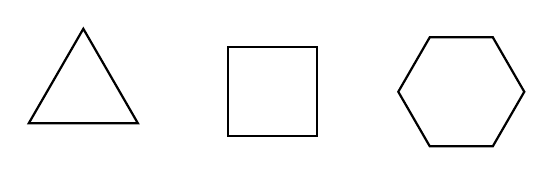
\begin{tikzpicture}[scale=0.8]
      \foreach \n/\x/\a in {3/0/90, 4/3/45, 6/6/0} {
        \draw[thick] ({\x + cos(\a)}, {sin(\a)})
          \foreach \k in {1, ..., \n} { -- ({\x + cos(\a + 360*\k/\n)}, {sin(\a + 360*\k/\n)}) } -- cycle;
      }
    \end{tikzpicture}
  \end{center}
  Die Gruppe $S_{E^2}(X)$ hat folgende Elemente:
  \begin{itemize}
    \item Rotationen um $\frac{2\pi k}{n}$, $k = 1, \dots, n$, insgesamt $n$ Stück.
    \item Spiegelungen:
      \begin{itemize}
        \item $n$ ungerade: Spiegelungen an Geraden durch eine Ecke und den Mittelpunkt der gegenüberliegenden Seite ($n$ Spiegelungen).
        \item $n$ gerade: Spiegelungen an Geraden durch gegenüberliegende Ecken und an Geraden durch die Mittelpunkte gegenüberliegender Seiten, insgesamt $n/2 + n/2 = n$ Spiegelungen.
      \end{itemize}
  \end{itemize}
  Also hat $S_{E^2}(X)$ genau $2n$ Elemente. Die Gruppe
  \[ D_{2n} \coloneqq S_{E^2}(X) \]
  heißt \emph{Diedergruppe} der Ordnung $2n$. Sie wird später abstrakter behandelt.
\end{example}


\subsection{Gruppen von Permutationen}

\begin{example}[Symmetrische und alternierende Gruppe]
  Sei $X$ eine Menge. Dann ist
  \[ \Sym(X) = \{ \alpha\colon X \to X \mid \alpha \text{ bijektiv} \} \]
  eine Gruppe unter Komposition. Es ist
  \[ S_n = \Sym(\{1, 2, \dots, n\}) \cong \Sym(X), \quad \text{falls } \lvert X \rvert = n. \]
  Die \emph{alternierende Gruppe}
  \[ A_n = \ker(\operatorname{sgn}) = \{ \sigma \in S_n \mid \operatorname{sgn}(\sigma) = 1 \} \]
  ist ein Normalteiler von $S_n$.
\end{example}

\section{Automorphismen und Konjugation}

\subsection{Automorphismen}

\begin{note}
  Ist $\varphi\colon G \to G'$ ein Gruppenhomomorphismus, so gilt
  \[ \varphi \text{ injektiv} \iff \ker\varphi = \{1\}. \]
  Statt $\{1\}$ schreiben wir auch kurz $1$.
\end{note}

\begin{definition}[Automorphismengruppe]\Theorem
  Die Menge
  \[ \Aut{G} \coloneqq \{\alpha\colon G \to G \mid \alpha \text{ Isomorphismus}\} \]
  der \emph{Automorphismen} von $G$ ist eine Gruppe unter Komposition.
\end{definition}

\begin{definition}[Charakteristische Untergruppe]\Theorem
  Eine Untergruppe $U \le G$ heißt \emph{charakteristisch} in $G$, falls $U\alpha = U$ für alle $\alpha \in \Aut{G}$. Wir schreiben dann $U \mathrel{\Char} G$.

  Eine Untergruppe $U \le G$ heißt \emph{vollinvariant}, falls $U\alpha \subseteq U$ für alle Homomorphismen $\alpha\colon G \to G$.
\end{definition}


\subsection{Konjugation}

\begin{definition}[Konjugation]\Theorem
  Sei $(G, \cdot)$ eine Gruppe und $g \in G$. Für $x \in G$ heißt
  \[ x^g \coloneqq g^{-1} x g \]
  die \emph{Konjugierte} von $x$ unter $g$. Für $H \subseteq G$ definieren wir $H^g \coloneqq \{h^g \mid h \in H\}$.
\end{definition}


Die \emph{Konjugationsabbildung} $c_g\colon G \to G$, $x \mapsto x^g$, ist ein Automorphismus von $G$.
Ist $H \le G$, so ist $H^g \le G$.
Für $N \le G$ gilt
\[ N \trianglelefteq G \iff N^g = N \quad \text{für alle } g \in G. \]


\begin{lemma}
  Ist $M \mathrel{\Char} N \trianglelefteq G$, so ist $M \trianglelefteq G$.
\end{lemma}
\begin{proof}
  Sei $g \in G$. Da $N \trianglelefteq G$, ist $N^{c_g} = N$. Wegen $c_g \in \Aut{G}$ ist $c_g|_N \in \Aut{N}$.
  Da $M \le N$, ist $M^{c_g} = M^{c_g|_N}$, und wegen $M \mathrel{\Char} N$ gilt $M^{c_g|_N} = M$.
  Also ist $M^{c_g} = M$.
\end{proof}


\begin{definition}[Normaler Abschluss]\Theorem
  Sei $(G, \cdot)$ eine Gruppe und $X \subseteq G$. Dann heißt
  \[ X^G \coloneqq \bigcap_{X \subseteq N \trianglelefteq G} N \]
  der \emph{normale Abschluss} von $X$ in $G$, also der kleinste Normalteiler von $G$, der $X$ enthält. Es gilt
  \[ X^G = \langle x^g \mid x \in X,\ g \in G \rangle. \]
\end{definition}


\section{Zyklische Gruppen}

\subsection{Die Ordnung eines Elements}

Sei $(G, \cdot)$ eine Gruppe.

\begin{definition}[Ordnung]\Theorem
  Für $x \in G$ heißt
  \[ \ord(x) = \begin{cases} \lvert \langle x \rangle \rvert, & \text{falls } \langle x \rangle \text{ endlich}, \\ \infty, & \text{sonst}, \end{cases} \]
  die \emph{Ordnung} von $x$. Man schreibt auch $\lvert x \rvert$ oder $o(x)$.
\end{definition}

\begin{definition}[Torsion]\Theorem
  $G$ heißt \emph{Torsionsgruppe}, falls $\ord(x)$ für alle $x \in G$ endlich ist.
  $G$ heißt \emph{torsionsfrei}, falls $o(x) = \infty$ für alle $x \in G \setminus \{1\}$.
\end{definition}


\begin{proposition}\label{prop:ordnung}
  Sei $x \in G$.
  \begin{enumerate}[label=(\roman*)]
    \item $\ord(x) = \infty \iff x^i \neq x^j$ für alle $i \neq j \in \Z$.
    \item Ist $n = \ord(x) < \infty$, so gilt $x^m = 1 \iff n \mid m$ für alle $m \in \Z$. Ferner ist
      \[ \langle x \rangle = \{1, x, x^2, \dots, x^{n-1}\}, \]
      und $1, x, \dots, x^{n-1}$ sind paarweise verschieden.
    \item Ist $\ord(x) = n < \infty$, so gilt
      \[ o(x^k) = \frac{n}{\ggT(n, k)}, \quad k \in \Z. \]
  \end{enumerate}
\end{proposition}
\begin{proof}
  Bei (i) ist \glqq$\Leftarrow$\grqq{} klar. Es gelte nun $x^l = x^m$ für $l, m \in \Z$ mit $l \neq m$ (dies existiert insbesondere, falls $o(x) < \infty$). Dann folgt
  \[ x^{l-m} = 1 = x^{-(l-m)}, \]
  also existiert ein $n \in \N_{\ge 1}$ mit $x^n = 1$. Wähle $n$ minimal mit dieser Eigenschaft.

  Ist $m \in \Z$, so können wir $m = qn + r$ mit $q, r \in \Z$ und $0 \le r \le n - 1$ schreiben. Dann gilt
  \[ x^m = \underbrace{(x^n)^q}_{= 1} \cdot x^r = x^r. \]
  Das ist wegen der Minimalität von $n$ genau dann gleich $1$, wenn $r = 0$ ist. Also gilt $x^m = 1 \iff n \mid m$.
  Außerdem ist stets $x^m = x^r \in \{1, x, \dots, x^{n-1}\}$, das heißt $\lvert \langle x \rangle \rvert \le n < \infty$, also $o(x) < \infty$.

  Wir zeigen nun, dass $1, x, \dots, x^{n-1}$ paarweise verschieden sind.
  Angenommen, $x^i = x^j$ für $0 \le i < j \le n-1$. Dann ist $x^{j-i} = 1$, nach der obigen Eigenschaft also $n \mid j - i$. Es ist aber $0 \le j - i \le n-1$, also $j - i = 0$, das heißt $j = i$.
  Damit sind (i) und (ii) gezeigt.

  Zu (iii): Sei $o(x) = n < \infty$ und $k \in \Z$. Dann gilt
  \[ \bigl(x^k\bigr)^{\frac{n}{\ggT(n, k)}} = \bigl(x^n\bigr)^{\frac{k}{\ggT(n, k)}} \overset{\text{(ii)}}{=} 1 \yf o\bigl(x^k\bigr) \le \frac{n}{\ggT(n, k)}. \]
  Sei $m \ge 1$ mit $x^{km} = \bigl(x^k\bigr)^m = 1$. Nach (ii) folgt $n \mid km$, also
  \[ \frac{n}{\ggT(n, k)} \;\Big|\; \frac{k}{\ggT(n, k)} \cdot m. \]
  Da $\frac{k}{\ggT(n, k)}$ teilerfremd zu $\frac{n}{\ggT(n, k)}$ ist, folgt mit dem Lemma von Euklid
  \[ \frac{n}{\ggT(n, k)} \;\Big|\; m, \]
  also $m \ge \frac{n}{\ggT(n, k)}$ und damit $o(x^k) = \frac{n}{\ggT(n, k)}$.
\end{proof}


\subsection{Untergruppen zyklischer Gruppen}

\begin{theorem}[Untergruppen zyklischer Gruppen]\Theorem
  Sei $G = \langle x \rangle$ und $H \le G$.
  \begin{enumerate}[label=(\roman*)]
    \item Ist $G$ unendlich, so ist $H$ unendlich zyklisch oder trivial.
    \item Ist $G$ endlich und $n = \lvert G \rvert$, so ist $H$ zyklisch und $\lvert H \rvert \mid n$.
      Umgekehrt existiert zu jedem Teiler $d$ von $n$ genau eine Untergruppe von $G$ der Ordnung $d$.
  \end{enumerate}
\end{theorem}
\begin{proof}
  (i) Wir zeigen zunächst, dass $H$ zyklisch ist. Für $H = 1$ ist das klar. Sei also $H \neq 1$.
  Dann existiert ein $s \in \Z$ mit $1 \neq x^s \in H$.
  Ist $s < 0$, so ist $-s > 0$ und $x^{-s} = (x^s)^{-1} \in H$. Wir können also $s > 0$ annehmen und $s$ minimal mit $1 \neq x^s \in H$ wählen.

  Zu zeigen ist $H = \langle x^s \rangle$. Klar ist $\langle x^s \rangle \subseteq H$.
  Sei $x^t \in H$. Schreibe $t = sq + r$ mit $q, r \in \Z$ und $0 \le r < s$. Dann gilt
  \[ H \ni x^t = \underbrace{(x^s)^q}_{\in H} x^r \yf x^r \in H. \]


\begin{ergaenzung}
  Wegen $0 \le r < s$ und der Wahl von $s$ ist $x^r = 1$, also $x^t = (x^s)^q \in \langle x^s \rangle$. Damit ist $H = \langle x^s \rangle$ zyklisch. Ist $G$ unendlich, so hat $x^s$ unendliche Ordnung, also ist $H$ unendlich zyklisch. Das zeigt (i).
  \end{ergaenzung}

  Zu (ii): Dass $H$ zyklisch ist, wurde oben gezeigt, und $\lvert H \rvert \mid \lvert G \rvert$ folgt aus dem Satz von Lagrange.

  Sei $d \ge 1$ ein Teiler von $n$. Dann gilt nach Proposition~\ref{prop:ordnung}
  \[ \bigl\lvert \langle x^{n/d} \rangle \bigr\rvert = o\bigl(x^{n/d}\bigr) = d. \]
  Sei nun $\langle x^k \rangle$ eine Untergruppe der Ordnung $d$. Dann gilt
  \begin{align*}
    &x^{kd} = (x^k)^d = 1 \yf n \mid k d \yf \tfrac{n}{d} \mid k \yf k = \tfrac{n}{d} \cdot \ell \text{ für ein } \ell \in \Z \\
    &\yf x^k = \bigl(x^{n/d}\bigr)^{\ell} \in \bigl\langle x^{n/d} \bigr\rangle \yf \langle x^k \rangle \le \bigl\langle x^{n/d} \bigr\rangle.
  \end{align*}
Beides sind Untergruppen der Ordnung $d$, also sind sie gleich.
\end{proof}

\begin{theorem}[Gruppen mit genau zwei Untergruppen]\Theorem
  Eine Gruppe $G$ hat genau dann genau zwei Untergruppen (nämlich $1$ und $G$), wenn $G$ zyklisch von Primzahlordnung ist.
\end{theorem}


\begin{proof}
  \glqq$\yf$\grqq: Hat $G$ genau zwei Untergruppen, so gilt $G \neq 1$. Wähle also $1 \neq x \in G$. Dann gilt
  \[ 1 \neq \langle x \rangle \le G \yf G = \langle x \rangle. \]
\begin{ergaenzung}
  $G$ ist endlich: Andernfalls hat $x$ unendliche Ordnung, also ist $x^2 \neq 1$. Wäre $x \in \langle x^2 \rangle$, etwa $x = x^{2m}$, so wäre $x^{2m-1} = 1$ mit $2m - 1 \neq 0$, ein Widerspruch. Also wäre $1 \neq \langle x^2 \rangle \neq G$ eine dritte Untergruppe.
  \end{ergaenzung}
  Nach Satz~\ref{Untergruppen zyklischer Gruppen} ist damit $\lvert G \rvert$ eine Primzahl.

  \glqq$\fy$\grqq: Satz von Lagrange.
\end{proof}

\subsection{Automorphismen zyklischer Gruppen}

\begin{theorem}[Automorphismen zyklischer Gruppen]\Theorem
  Sei $G$ eine zyklische Gruppe.
  \begin{enumerate}[label=(\roman*)]
    \item Ist $G$ unendlich, so hat $G$ genau zwei Automorphismen, nämlich $\id_G$ und $G \to G$, $g \mapsto g^{-1}$. Insbesondere ist $\Aut{G}$ zyklisch der Ordnung $2$.
    \item Sei $\lvert G \rvert = n < \infty$. Dann ist
      \[ \Aut{G} = \{\alpha_k \mid 1 \le k < n,\ \ggT(k, n) = 1\}, \quad \text{wobei } \alpha_k\colon G \to G,\ g \mapsto g^k. \]
      Außerdem ist die Abbildung
      \[ \Theta\colon \Z_n^* \to \Aut{G}, \quad n\Z + k \mapsto \alpha_k, \]
      ein Isomorphismus. Insbesondere ist $\lvert \Aut{G} \rvert = \varphi(n)$.
  \end{enumerate}
  Dabei ist $\Z_n = \Z / n\Z$, $\Z_n^*$ die Gruppe der invertierbaren Elemente in $\Z_n$ und $\varphi$ die Eulersche $\varphi$-Funktion.
\end{theorem}


\begin{proof}
  Sei $G = \langle x \rangle$ und $\alpha \in \Aut{G}$. Für $\ell \in \Z$ gilt $x^\ell \alpha = (x\alpha)^\ell$. Daher ist $\alpha$ durch $x\alpha$ eindeutig bestimmt. Außerdem ist $G = \langle x\alpha \rangle$.

  (i) Sei zunächst $G$ unendlich. Dann sind $x$ und $x^{-1}$ die einzigen Erzeuger von $G$, also ist $x\alpha = x$ oder $x\alpha = x^{-1}$. Weil $G$ abelsch ist, ist $G \to G$, $g \mapsto g^{-1}$, ein Automorphismus. Daraus folgt (i).

  (ii) Sei $\lvert G \rvert = n < \infty$. Dann ist $o(x\alpha) = o(x) = n$. Schreibe $x\alpha = x^k$. Nach Proposition~\ref{prop:ordnung} gilt
  \[ n = o(x^k) = \frac{n}{\ggT(k, n)} \yf \ggT(k, n) = 1. \]
  Ist umgekehrt $\ggT(k, n) = 1$, so existieren nach dem Lemma von Bézout $u, v \in \Z$ mit
  \[ uk + vn = 1, \quad \text{d.\,h. } uk \equiv 1 \bmod n. \]
  Daraus folgt
  \[ (x^u)^k = (x^k)^u = x^{uk} = x. \]
  Wir können dabei $1 \le u < n$ wählen. Dann ist $\alpha_u$ die Umkehrabbildung zu $\alpha_k$, also ist $\alpha_k$ bijektiv. Da $G$ abelsch ist, ist $\alpha_k$ ein Homomorphismus, also $\alpha_k \in \Aut{G}$.


  Wegen $g^{k\ell} = (g^k)^\ell$ gilt
  \[ \alpha_{k\ell} = \alpha_k \alpha_\ell \quad \text{für } k, \ell \in \{1, \dots, n-1\}. \]
  Also ist $\Theta$ ein Homomorphismus. Nach dem eben Gezeigten ist $\Theta$ surjektiv.

  Ist $x^k = x^\ell$ mit $\ggT(n, k) = \ggT(n, \ell) = 1$, so sind $k + n\Z$ und $\ell + n\Z$ invertierbar, etwa $\bar\ell + n\Z = (\ell + n\Z)^{-1}$. Dann gilt
  \begin{align*}
    x^{k\bar\ell} = x &\yf x^{k\bar\ell - 1} = 1 \yf n \mid k\bar\ell - 1 \\
    &\yf (\ell + n\Z)^{-1} = \bar\ell + n\Z = (k + n\Z)^{-1} \yf \ell + n\Z = k + n\Z.
  \end{align*}
  Also ist $\Theta$ injektiv.
\end{proof}

\section{Operationen von Gruppen}

\subsection{Definition und Beispiele}

Sei $G$ stets eine Gruppe und $X$ eine Menge.

\begin{definition}[Operation]\Theorem
  Eine \emph{Operation} von $G$ auf $X$ (von rechts) ist eine Abbildung
  \[ X \times G \to X, \quad (x, g) \mapsto xg, \]
  sodass
  \begin{align*}
    x 1_G &= x && \text{für alle } x \in X, \\
    (xg)h &= x(gh) && \text{für alle } x \in X,\ g, h \in G.
  \end{align*}
\end{definition}

\begin{example}
  \begin{itemize}
    \item $G$ operiert auf sich selbst durch \glqq Rechtsmultiplikation\grqq, d.\,h. die Multiplikation
      \[ G \times G \to G, \quad (x, g) \mapsto x \cdot g, \]
      ist eine Operation von $G$ auf $G$.
    \item $G$ operiert auf sich selbst durch \glqq Linksmultiplikation mit Inversen\grqq. Genauer ist
      \[ G \times G \to G, \quad (x, g) \mapsto \underbrace{g^{-1} x}_{\eqqcolon x \circ g}, \]
      eine Operation:
      \begin{align*}
        x \circ 1_G &= 1_G^{-1} x = 1_G x = x, \\
        (x \circ g) \circ h &= h^{-1} (g^{-1} x) = (h^{-1} g^{-1}) x = (gh)^{-1} x = x \circ (gh).
      \end{align*}
    \item $G$ operiert auf $G$ durch Konjugation, d.\,h.
      \[ G \times G \to G, \quad (x, g) \mapsto x^g = g^{-1} x g, \]
      ist eine Operation:
      \begin{align*}
        x^1 &= x, \\
        (x^g)^h &= h^{-1} (g^{-1} x g) h = (h^{-1} g^{-1})\, x\, (gh) = (gh)^{-1}\, x\, (gh) = x^{gh}.
      \end{align*}
  \end{itemize}
\end{example}

\begin{note}
  Ist $X \times G \to X$, $(x, g) \mapsto xg$, eine Operation, so operiert $G$ auch auf der Potenzmenge $\pot(X)$ von $X$, d.\,h.
  \[ \pot(X) \times G \to \pot(X), \quad (A, g) \mapsto Ag \coloneqq \{ag : a \in A\}, \]
  ist eine Operation.

  Ist $B \subseteq X$ mit $Bg = B$ für alle $g \in G$, so operiert $G$ auf $B$, denn die Einschränkung der Operation $X \times G \to X$ zu einer Abbildung $B \times G \to B$ ist eine Operation.
\end{note}

\begin{example}
  \begin{itemize}
    \item $G$ operiert auf jedem Normalteiler von $G$ durch Konjugation.
    \item $G$ operiert auf $\pot(G)$ durch Rechtsmultiplikation, durch Linksmultiplikation mit Inversen und durch Konjugation.
    \item Ist $H \le G$, so ist $H^g \le G$ für alle $g \in G$. Also operiert $G$ auf der Menge der Untergruppen von $G$ durch Konjugation.
    \item Ist $H \le G$ und sind $x, g \in G$, so ist $(Hx)g = H(xg)$ wieder eine Rechtsnebenklasse. Das heißt, $G$ operiert auf den Rechtsnebenklassen von $H$ durch Rechtsmultiplikation.

      Genauso ist $g^{-1}(xH) = (g^{-1}x)H$. Daher operiert $G$ auf den Linksnebenklassen von $H$ in $G$ durch Linksmultiplikation mit Inversen:
      \[ \{xH : x \in G\} \times G \to \{xH : x \in G\}, \quad (xH, g) \mapsto g^{-1} x H, \]
      ist eine Operation.
  \end{itemize}
\end{example}

\subsection{Operationen und Homomorphismen}

Ist $X \times G \to X$, $(x, g) \mapsto xg$, eine Operation, so ist für jedes $g \in G$
\[ \pi_g\colon X \to X, \quad x \mapsto xg, \]
eine Bijektion, denn $\pi_{g^{-1}}$ ist die Umkehrabbildung: $(xg)g^{-1} = x(gg^{-1}) = x 1_G = x$, und genauso $(xg^{-1})g = x$. Also ist $\pi_g \in \Sym(X)$.

Sei $\pi\colon G \to \Sym(X)$, $g \mapsto \pi_g$. Dann ist $\pi$ ein Homomorphismus, d.\,h. $\pi_{gh} = \pi_g \pi_h$, denn für $x \in X$ gilt
\[ x \pi_{gh} = x(gh) = (xg)h = x \pi_g \pi_h. \]

Ist umgekehrt $\varphi\colon G \to \Sym(X)$ ein Homomorphismus, so ist
\[ X \times G \to X, \quad (x, g) \mapsto \overbrace{x(\underbrace{g\varphi}_{\in \Sym(X)})}^{\eqqcolon x \cdot g}, \]
eine Operation:
\begin{align*}
  x \cdot 1_G &= x(1_G \varphi) = x \id_X = x, \\
  (x \cdot g) \cdot h &= x(g\varphi)(h\varphi) \overset{\varphi \text{ Hom.}}{=} x\bigl((gh)\varphi\bigr) = x \cdot (gh).
\end{align*}
Bildet man für diese Operation die Abbildung $\pi$ wie oben, so gilt $\pi = \varphi$.

\subsection{Bahnen und Stabilisatoren}

\begin{definition}[Bahn und Stabilisator]\Theorem
  Sei $X \times G \to X$, $(x, g) \mapsto xg$, eine Operation. Für $x \in X$ heißt
  \begin{itemize}
    \item $xG \coloneqq \{xg : g \in G\}$ die \emph{Bahn} von $x$ unter $G$,
    \item $G_x \coloneqq \{g \in G \mid xg = x\}$ der \emph{Stabilisator} von $x$ in $G$.
  \end{itemize}
\end{definition}

\begin{lemma}[Stabilisatoren]\Theorem
  Sei $X \times G \to X$ eine Operation, $x \in X$ und $g \in G$.
  \begin{enumerate}[label=(\roman*)]
    \item $G_x$ ist eine Untergruppe von $G$.
    \item $G_x^{\,g} = G_{xg}$.
  \end{enumerate}
\end{lemma}

\begin{proof}
  (i) Wegen $x \cdot 1_G = x$ ist $1_G \in G_x$. Für $g, h \in G_x$ gilt
  \[ xg = x,\ xh = x \yf x(gh) = (xg)h = xh = x \yf gh \in G_x. \]
  Außerdem ist $x g^{-1} = (xg) g^{-1} = x(g g^{-1}) = x 1_G = x$, also $g^{-1} \in G_x$.

  (ii) Es gilt
  \begin{align*}
    G_{xg} &= \{a \in G : xga = xg\} = \{a \in G : xgag^{-1} = x\} = \{a \in G : gag^{-1} \in G_x\} \\
    &= \{a \in G : a \in g^{-1} G_x g\} = G_x^{\,g}. \qedhere
  \end{align*}
\end{proof}

\begin{lemma}[Bahn-Stabilisator-Lemma]\Theorem
  Sei $X \times G \to X$ eine Operation und $x \in X$. Dann ist die Abbildung
  \[ \{G_x h : h \in G\} \to xG, \quad G_x h \mapsto xh, \]
  wohldefiniert und eine Bijektion. Insbesondere ist
  \[ \lvert G : G_x \rvert = \lvert xG \rvert, \]
  d.\,h. die Länge der Bahn ist gleich dem Index des Stabilisators.
\end{lemma}


\begin{proof}
  Für $g, h \in G$ gilt
  \[ G_x h = G_x g \iff hg^{-1} \in G_x \iff x(hg^{-1}) = x \iff x(hg^{-1})g = xg \iff xh = xg. \]
  Die Richtung \glqq$\yf$\grqq{} bedeutet, dass die Abbildung wohldefiniert ist, die Richtung \glqq$\fy$\grqq{} zeigt die Injektivität. Die Surjektivität folgt aus der Definition der Bahn.
\end{proof}

\begin{definition}[Transitive Operation]\Theorem
  Eine Operation $X \times G \to X$ heißt \emph{transitiv}, falls ein $x \in X$ mit $xG = X$ existiert. Wir sagen dann auch, dass $G$ \emph{transitiv} auf $X$ operiert.
\end{definition}

\begin{note}
  Ist die Operation transitiv, so gilt $yG = X$ für alle $y \in X$. Ist nämlich $xG = X$, so ist $y = xh$ für ein $h \in G$, und damit
  \[ yG = \{(xh)g : g \in G\} = \{x(hg) : g \in G\} = \{xa : a \in \underbrace{hG}_{= G}\} = xG = X. \]
  Für eine transitive Operation besagt das Bahn-Stabilisator-Lemma daher
  \[ \lvert X \rvert = \lvert G : G_x \rvert \quad \text{für alle } x \in X. \]
\end{note}


\section{Diedergruppen}

\subsection{Produkte von Untergruppen}

Für Teilmengen $A, B \subseteq G$ schreiben wir
\[ AB \coloneqq \{ab \mid a \in A,\ b \in B\}, \qquad A^{-1} \coloneqq \{a^{-1} \mid a \in A\}. \]


\begin{ergaenzung}

\begin{lemma}[Produkt von Untergruppen]\Theorem
  Seien $A, B \le G$. Dann gilt
  \[ AB \le G \iff AB = BA. \]
\end{lemma}

\begin{proof}
  \glqq$\yf$\grqq: Ist $AB \le G$, so ist $AB = (AB)^{-1} = B^{-1}A^{-1} = BA$.

  \glqq$\fy$\grqq: Sei $AB = BA$. Wegen $1 = 1 \cdot 1 \in AB$ ist $AB \neq \emptyset$. Es gilt
  \[ (AB)^{-1} = B^{-1}A^{-1} = BA = AB \]
  und
  \[ (AB)(AB) = A(BA)B = A(AB)B = (AA)(BB) = AB, \]
  da $A, B \le G$. Also ist $AB$ unter Produkten und Inversen abgeschlossen, d.\,h. $AB \le G$.
\end{proof}

\begin{lemma}
  Ist $A \le G$ und $N \trianglelefteq G$, so gilt $AN = NA \le G$.
\end{lemma}

\begin{proof}
  Nach dem vorigen Lemma genügt es, $AN = NA$ zu zeigen. Da $N \trianglelefteq G$, ist $aN = Na$ für alle $a \in A$, also
  \[ AN = \bigcup_{a \in A} aN = \bigcup_{a \in A} Na = NA. \qedhere \]
\end{proof}
\end{ergaenzung}


\Needspace{10\baselineskip}
\subsection{Normalisator und semidirektes Produkt}

\begin{ergaenzung}
\begin{definition}[Normalisator]\Theorem
  Sei $U \le G$. Dann heißt
  \[ N_G(U) \coloneqq \{g \in G \mid U^g = U\} \]
  der \emph{Normalisator} von $U$ in $G$. Es gilt $U \le N_G(U) \le G$ und
  \[ U \trianglelefteq G \iff N_G(U) = G. \]
\end{definition}

\begin{definition}[Involution]\Theorem
  Ein Element $s \in G$ heißt \emph{Involution}, falls $o(s) = 2$.
\end{definition}
\end{ergaenzung}

\begin{ergaenzung}
\begin{definition}[Semidirektes Produkt]\Theorem
  Seien $A, N \le G$. Dann heißt $G$ ein \emph{(internes) semidirektes Produkt} von $A$ mit $N$, falls
  \[ G = AN, \qquad A \cap N = 1, \qquad N \trianglelefteq G. \]
  Wir schreiben dann $G = A \ltimes N$.
\end{definition}


\begin{note}
  Ist $G = A \ltimes N$, so lässt sich jedes Element von $G$ eindeutig als $an$ mit $a \in A$ und $n \in N$ schreiben, und es gilt
  \[ (a_1 n_1)(a_2 n_2) = (a_1 a_2)\bigl(n_1^{a_2} n_2\bigr). \]
  Das legt die folgende Konstruktion nahe.
\end{note}

\begin{definition}[Externes semidirektes Produkt]\Theorem
  Seien $A$ und $N$ Gruppen, und $A$ operiere auf $N$ (von rechts) durch Automorphismen, d.\,h. es gibt eine Abbildung $N \times A \to N$, $(n, a) \mapsto n^a$, mit
  \[ n^1 = n, \qquad (n^a)^b = n^{ab}, \qquad (nm)^a = n^a m^a \]
  für alle $n, m \in N$ und $a, b \in A$. Dann ist $A \times N$ mit der Multiplikation
  \[ (a_1, n_1) \cdot (a_2, n_2) \coloneqq \bigl(a_1 a_2,\ n_1^{a_2} n_2\bigr) \]
  eine Gruppe, das \emph{(externe) semidirekte Produkt} von $A$ mit $N$. Sie ist das interne semidirekte Produkt ihrer Untergruppen $\bar{A} \coloneqq \{(a, 1) \mid a \in A\} \cong A$ und $\bar{N} \coloneqq \{(1, n) \mid n \in N\} \cong N$, und für $n \in N$, $a \in A$ gilt $(1, n)^{(a, 1)} = (1, n^a)$.
\end{definition}
\end{ergaenzung}

\subsection{Diedergruppen}

\begin{ergaenzung}
\begin{lemma}[Diederbedingung]\Theorem
  Sei $G$ eine Gruppe. Dann sind äquivalent:
  \begin{enumerate}[label=(\roman*)]
    \item Es gibt Involutionen $s \neq t$ in $G$ mit $G = \langle s, t \rangle$.
    \item Es gibt $t, x \in G$ mit $x \neq 1$, $o(t) = 2$, $x^t = x^{-1}$ und $G = \langle t \rangle \ltimes \langle x \rangle$.
  \end{enumerate}
\end{lemma}
\end{ergaenzung}


\begin{ergaenzung}
\begin{center}
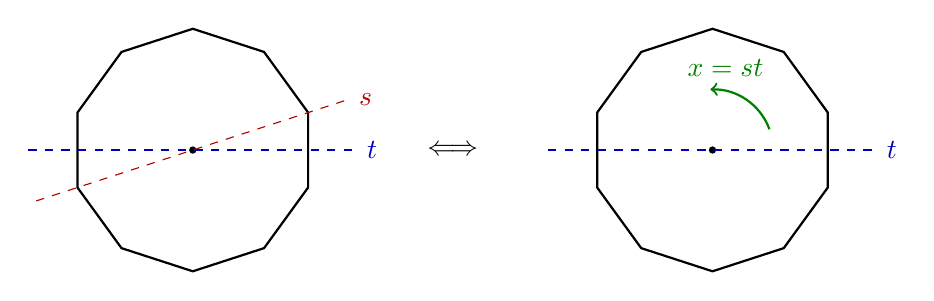
\begin{tikzpicture}[scale=1.1]
  \foreach \cx in {0, 6} {
    \draw[thick] ({\cx + 1.4*cos(18)}, {1.4*sin(18)})
      \foreach \k in {1, ..., 10} { -- ({\cx + 1.4*cos(18 + 36*\k)}, {1.4*sin(18 + 36*\k)}) } -- cycle;
    \fill (\cx, 0) circle (1.2pt);
  }
\draw[blue!70!black, dashed] (-1.9, 0) -- (1.9, 0) node[right] {$t$};
  \draw[red!70!black, dashed] ({-1.9*cos(18)}, {-1.9*sin(18)}) -- ({1.9*cos(18)}, {1.9*sin(18)}) node[right] {$s$};
  \node at (3, 0) {$\iff$};
\draw[blue!70!black, dashed] (4.1, 0) -- (7.9, 0) node[right] {$t$};
  \draw[->, thick, green!50!black] ({6 + 0.7*cos(20)}, {0.7*sin(20)}) arc (20:92:0.7);
  \node[green!50!black] at (6.15, 0.95) {$x = st$};
\end{tikzpicture}
\end{center}
\end{ergaenzung}


\begin{ergaenzung}
\begin{proof}
  \glqq(i) $\yf$ (ii)\grqq: Sei $G = \langle s, t \rangle$ mit $o(s) = o(t) = 2$ und $s \neq t$. Setze $x \coloneqq st$. Wegen $s \neq t$ ist $x \neq 1$. Da $t = t^{-1}$ und $s = s^{-1}$, gilt
  \[ x^t = t^{-1} x t = tstt = ts = t^{-1}s^{-1} = (st)^{-1} = x^{-1}. \]
  Also ist $\langle x \rangle^t = \langle x^t \rangle = \langle x \rangle$, d.\,h. $t \in N_G(\langle x \rangle)$, und offensichtlich ist $x \in N_G(\langle x \rangle)$. Wegen $s = xt$ ist
  \[ G = \langle s, t \rangle = \langle x, t \rangle \le N_G(\langle x \rangle), \]
  also $\langle x \rangle \trianglelefteq G$. Nach dem Lemma über Produkte von Untergruppen ist $\langle t \rangle \langle x \rangle \le G$, und da diese Untergruppe $x$ und $t$ enthält, ist $\langle t \rangle \langle x \rangle = \langle x, t \rangle = G$.

  Es bleibt $\langle t \rangle \cap \langle x \rangle = 1$ zu zeigen. Angenommen, nicht. Wegen $\lvert \langle t \rangle \rvert = 2$ ist dann $t \in \langle x \rangle$. Dann ist $x^t = x$, also $x = x^{-1}$, d.\,h. $x^2 = 1$. Da $x \neq 1$, ist $\langle x \rangle = \{1, x\}$ und damit $t = x = st$, also $s = 1$, ein Widerspruch zu $o(s) = 2$. Also ist $G = \langle t \rangle \ltimes \langle x \rangle$.


  \glqq(ii) $\yf$ (i)\grqq: Sei $G = \langle t \rangle \ltimes \langle x \rangle$ mit $o(t) = 2$, $x \neq 1$ und $x^t = x^{-1}$. Setze $s \coloneqq xt$. Wegen $\langle t \rangle \cap \langle x \rangle = 1$ ist $t \neq x^{-1}$, also $s \neq 1$, und wegen $x \neq 1$ ist $s \neq t$. Da $t = t^{-1}$, gilt
  \[ s^2 = xtxt = x\,(t^{-1}xt) = x x^t = x x^{-1} = 1, \]
  also $o(s) = 2$. Schließlich ist $G = \langle t, x \rangle = \langle t, xt \rangle = \langle s, t \rangle$.
\end{proof}
\end{ergaenzung}


\begin{ergaenzung}
\begin{definition}[Diedergruppe]\Theorem
  Eine Gruppe, die eine der beiden äquivalenten Bedingungen des Lemmas erfüllt, heißt \emph{Diedergruppe}. Sei $G = \langle t \rangle \ltimes \langle x \rangle$ wie in (ii).
  \begin{itemize}
    \item Ist $o(x) = n < \infty$, so schreiben wir $D_{2n}$ für $G$ und nennen $G$ die \emph{Diedergruppe der Ordnung $2n$}. Sie ist die Symmetriegruppe des regulären $n$-Ecks aus Abschnitt~3.
    \item Ist $o(x) = \infty$, d.\,h. $\langle x \rangle \cong (\Z, +)$, so schreiben wir $D_\infty$ für $G$ und nennen $G$ die \emph{unendliche Diedergruppe}. Dass sie existiert, sieht man am externen semidirekten Produkt von $\langle t \rangle \cong \Z/2\Z$ mit $(\Z, +)$, wobei $t$ durch $n \mapsto -n$ operiert.
  \end{itemize}
\end{definition}
\end{ergaenzung}


\section{Freie Gruppen}

\subsection{Definition und Existenz}

\begin{definition}[Freie Gruppe]\Theorem
  Sei $F$ eine Gruppe, $X \neq \emptyset$ eine Menge und $\sigma\colon X \to F$ eine Abbildung. Dann heißt $F$, genauer $(F, \sigma)$, \emph{frei auf $X$}, falls für jede Gruppe $G$ und für jede Abbildung $\alpha\colon X \to G$ genau ein Homomorphismus $\beta\colon F \to G$ mit $\sigma\beta = \alpha$ existiert.
  \[
    \begin{tikzcd}
      & F \arrow[dashed]{dr}{\exists!\, \beta} & \\
      X \arrow{ur}{\sigma} \arrow[swap]{rr}{\alpha} & & G
    \end{tikzcd}
  \]
  Eine Gruppe, die frei auf irgendeiner Menge ist, heißt \emph{freie Gruppe}.
\end{definition}


\begin{note}
  Ist $(F, \sigma)$ frei auf $X$, so ist $\sigma$ injektiv.
\end{note}

\begin{proof}
  Seien $x_1 \neq x_2 \in X$. Wähle eine Gruppe $G \neq 1$ und $g_1 \neq g_2 \in G$ sowie eine Abbildung $\alpha\colon X \to G$ mit $x_i\alpha = g_i$ für $i = 1, 2$. Dann existiert $\beta\colon F \to G$ mit $\sigma\beta = \alpha$. Wäre $x_1\sigma = x_2\sigma$, so wäre
  \[ g_1 = x_1\alpha = x_1\sigma\beta = x_2\sigma\beta = x_2\alpha = g_2, \]
  ein Widerspruch.
\end{proof}


Wir werden später sehen, dass $\langle \im\sigma \rangle = F$ gilt.
Ist $(F, \sigma)$ frei auf $X$, so ist $(F, \text{Inklusion})$ frei auf $\im\sigma$.

\begin{theorem}[Existenz freier Gruppen]\Theorem
  Sei $X \neq \emptyset$ eine Menge. Dann existieren eine Gruppe $F$ und eine Abbildung $\sigma\colon X \to F$, sodass $(F, \sigma)$ frei auf $X$ ist und $F = \langle \im\sigma \rangle$.
\end{theorem}


\begin{proof}
  Wähle eine zu $X$ disjunkte Menge $X^{-1}$ mit $\lvert X^{-1} \rvert = \lvert X \rvert$ und eine Bijektion $X \to X^{-1}$, $x \mapsto x^{-1}$. Dabei ist $x^{-1}$ zunächst nur ein neues Symbol.

  \textit{Wörter.} Ein \emph{Wort} in $X$ ist eine endliche Folge von Symbolen aus $X \cup X^{-1}$, geschrieben als
  \[ w = x_1^{\varepsilon_1} \cdots x_r^{\varepsilon_r} \quad \text{mit } r \ge 0,\ x_i \in X \text{ und } \varepsilon_i \in \{1, -1\} \text{ für alle } i = 1, \dots, r. \]
  Ist $r = 0$, so meinen wir das \emph{leere Wort} $1$.
Das Produkt zweier Wörter in $X$ ist einfach die Konkatenation: Ist $w = x_1^{\varepsilon_1} \cdots x_r^{\varepsilon_r}$ und $v = y_1^{\delta_1} \cdots y_s^{\delta_s}$, so ist
  \[ wv = x_1^{\varepsilon_1} \cdots x_r^{\varepsilon_r} y_1^{\delta_1} \cdots y_s^{\delta_s}. \]
  Dabei vereinbaren wir $w1 = w$ und $1w = w$. Das \emph{Inverse} von $w$ ist
  \[ w^{-1} \coloneqq x_r^{-\varepsilon_r} \cdots x_1^{-\varepsilon_1}, \qquad 1^{-1} = 1. \]

  \textit{Die Gruppe $F$.} Sei $S$ die Menge der Wörter in $X$. Wir definieren eine Äquivalenzrelation auf $S$: Es sei $w \sim v$, wenn wir durch endlich viele Hintereinanderausführungen der folgenden Operationen von $w$ nach $v$ gelangen können:
  \begin{enumerate}[label=(\alph*)]
    \item Einfügen von $xx^{-1}$ oder $x^{-1}x$ ($x \in X$) als aufeinanderfolgende Elemente an beliebiger Stelle in das Wort,
    \item Streichen von $xx^{-1}$ und $x^{-1}x$.
  \end{enumerate}
  Dann ist $\sim$ eine Äquivalenzrelation. Wir schreiben $[w]$ für die Äquivalenzklasse von $w$ und setzen
  \[ F \coloneqq S/{\sim} \coloneqq \{ [w] : w \in S \}, \qquad [w] \cdot [v] \coloneqq [wv]. \]
  Das ist wohldefiniert: Ist $w \sim w'$ und $v \sim v'$, so ist $wv \sim w'v'$. Es gilt $[w] \cdot [1] = [w] = [1] \cdot [w]$ und
  \[ [w] \cdot [w^{-1}] = [ww^{-1}] = [1]. \]
  Da die Konkatenation assoziativ ist, ist auch das Produkt auf $F$ assoziativ. Also ist $F$ eine Gruppe.

  \textit{$(F, \sigma)$ ist frei auf $X$.} Sei $\sigma\colon X \to F$, $x \mapsto [x]$. Sei $G$ eine Gruppe und $\alpha\colon X \to G$ eine Abbildung. Zu zeigen ist, dass genau ein Homomorphismus $\beta\colon F \to G$ mit $\sigma\beta = \alpha$ existiert.

  Definiere zunächst
  \[ \bar\beta\colon S \to G, \quad x_1^{\varepsilon_1} \cdots x_r^{\varepsilon_r} \mapsto (x_1\alpha)^{\varepsilon_1} \cdots (x_r\alpha)^{\varepsilon_r}. \]
  Ist $w \sim v$, so gilt $w\bar\beta = v\bar\beta$. Also können wir
  \[ \beta\colon F \to G, \quad [w] \mapsto w\bar\beta, \]
  definieren. Nach Definition von $\bar\beta$ gilt
  \[ ([w] \cdot [v])\beta = [wv]\beta = (wv)\bar\beta = (w\bar\beta)(v\bar\beta) = ([w]\beta) \cdot ([v]\beta), \]
  also ist $\beta$ ein Homomorphismus. Für $x \in X$ gilt nach Definition von $\bar\beta$
  \[ x\sigma\beta = [x]\beta = x\bar\beta = x\alpha, \]
  also $\sigma\beta = \alpha$.

  Es bleibt zu zeigen, dass $\beta$ eindeutig ist. Sei $\gamma\colon F \to G$ ein Homomorphismus mit $\sigma\gamma = \alpha$. Offensichtlich ist $F = \langle [x] : x \in X \rangle = \langle \im\sigma \rangle$. Wegen $\sigma\gamma = \alpha = \sigma\beta$ ist $\gamma|_{\im\sigma} = \beta|_{\im\sigma}$, also $\gamma = \beta$.
\end{proof}


\subsection{Reduzierte Wörter und Normalform}

Betrachte die Konstruktion oben. Ist $w = x_1^{\varepsilon_1} \cdots x_r^{\varepsilon_r}$, so ist
\[ [w] = [x_1^{\varepsilon_1}] \cdots [x_r^{\varepsilon_r}] = [x_1]^{\varepsilon_1} \cdots [x_r]^{\varepsilon_r}. \]
Wir wollen jedes Element von $F$ so einfach wie möglich als ein solches Produkt darstellen, in dem sich nichts mehr \glqq wegkürzen\grqq{} lässt.

\begin{definition}[Reduziertes Wort]\Theorem
  Ein Wort $w$ in $X$ heißt \emph{reduziert}, falls es kein Teilwort der Form $xx^{-1}$ oder $x^{-1}x$ mit $x \in X$ besitzt.
\end{definition}

Offensichtlich existiert in jeder Äquivalenzklasse $[w] \in F$ ein reduziertes Wort.

\begin{theorem}[Eindeutigkeit reduzierter Wörter]\Theorem
  Jede Äquivalenzklasse von Wörtern in $X$ (wie oben konstruiert) enthält genau ein reduziertes Wort.
\end{theorem}


\begin{proof}
  Sei $R$ die Menge der reduzierten Wörter in $X$. Wir konstruieren mit der universellen Eigenschaft von $F$ einen Homomorphismus $\theta\colon F \to \Sym(R)$.

  Für $u \in X \cup X^{-1}$ definiere die Funktion $u'\colon R \to R$ durch
  \[
    (x_1^{\varepsilon_1} \cdots x_r^{\varepsilon_r})u' \coloneqq
    \begin{cases}
      x_1^{\varepsilon_1} \cdots x_r^{\varepsilon_r} u, & u \neq x_r^{-\varepsilon_r}, \\
      x_1^{\varepsilon_1} \cdots x_{r-1}^{\varepsilon_{r-1}}, & u = x_r^{-\varepsilon_r},
    \end{cases}
  \]
  für reduzierte Wörter $x_1^{\varepsilon_1} \cdots x_r^{\varepsilon_r}$.

  \textit{Es gilt $u'(u^{-1})' = \id_R$:} Ist $u \neq x_r^{-\varepsilon_r}$, so gilt
  \[ (x_1^{\varepsilon_1} \cdots x_r^{\varepsilon_r})u'(u^{-1})' = (x_1^{\varepsilon_1} \cdots x_r^{\varepsilon_r} u)(u^{-1})' = x_1^{\varepsilon_1} \cdots x_r^{\varepsilon_r}. \]
  Ist $u = x_r^{-\varepsilon_r}$, so gilt $u^{-1} = x_r^{\varepsilon_r} \neq x_{r-1}^{-\varepsilon_{r-1}}$, da $x_1^{\varepsilon_1} \cdots x_r^{\varepsilon_r}$ reduziert ist. Also ist
  \[ (x_1^{\varepsilon_1} \cdots x_r^{\varepsilon_r})u'(u^{-1})' = (x_1^{\varepsilon_1} \cdots x_{r-1}^{\varepsilon_{r-1}})(u^{-1})' = x_1^{\varepsilon_1} \cdots x_{r-1}^{\varepsilon_{r-1}} \underbrace{x_r^{\varepsilon_r}}_{= u^{-1}}. \]
  Also ist $u'(u^{-1})' = \id_R$ und genauso $(u^{-1})'u' = \id_R$. Damit ist $u'$ eine Bijektion, d.\,h. $u' \in \Sym(R)$.

  Also ist $\alpha\colon X \to \Sym(R)$, $x \mapsto x'$, wohldefiniert. Wegen der universellen Eigenschaft von $F$ existiert ein Homomorphismus $\theta\colon F \to \Sym(R)$ mit $\sigma\theta = \alpha$, also
  \[ [x]\theta = x\alpha = x' \quad \text{für } x \in X. \]
  \[
    \begin{tikzcd}
      & F = S/{\sim} \arrow[dashed]{dr}{\exists!\, \theta} & \\
      X \arrow{ur}{\sigma} \arrow[swap]{rr}{\alpha} & & \Sym(R)
    \end{tikzcd}
  \]

  Seien nun $v, w \in R$ mit $v \sim w$. Zu zeigen ist $v = w$. Aus $[v] = [w]$ folgt $[v]\theta = [w]\theta \in \Sym(R)$. Sei $v = x_1^{\varepsilon_1} \cdots x_r^{\varepsilon_r}$. Dann ist $[v] = [x_1^{\varepsilon_1}] \cdots [x_r^{\varepsilon_r}]$ und
  \[ [v]\theta = \bigl([x_1^{\varepsilon_1}]\theta\bigr) \cdots \bigl([x_r^{\varepsilon_r}]\theta\bigr) = (x_1^{\varepsilon_1})' \cdots (x_r^{\varepsilon_r})' \in \Sym(R). \]
  Wende diese Funktion auf das leere Wort $1$ an:
  \[ 1\bigl([v]\theta\bigr) = 1\,(x_1^{\varepsilon_1})' \cdots (x_r^{\varepsilon_r})' = x_1^{\varepsilon_1} (x_2^{\varepsilon_2})' \cdots (x_r^{\varepsilon_r})' = x_1^{\varepsilon_1} x_2^{\varepsilon_2} \cdots x_r^{\varepsilon_r} = v. \]
  Hier geht ein, dass $v$ reduziert ist. Also ist $1([v]\theta) = v$ und genauso $1([w]\theta) = w$. Nach Annahme gilt $[v]\theta = [w]\theta$, also $v = w$.
\end{proof}

\paragraph{Normalform.}
Nach dem Satz kann jedes Element von $F$ (wie oben konkret konstruiert) eindeutig in der Form $[w]$ mit einem reduzierten Wort $w$ geschrieben werden, etwa
\[ w = x_1^{\varepsilon_1} \cdots x_r^{\varepsilon_r} \quad \text{mit } r \ge 0,\ x_i \in X,\ \varepsilon_i = \pm 1. \]
Dann ist $[w] = [x_1]^{\varepsilon_1} \cdots [x_r]^{\varepsilon_r}$. Indem wir hintereinander auftretende Terme mit demselben Element $x_i$ zusammenmultiplizieren, gelangen wir zu einem Ausdruck der Form
\[ [w] = [y_1]^{l_1} \cdots [y_s]^{l_s} \quad \text{mit } s \ge 0,\ l_i \in \Z \setminus \{0\},\ y_i \neq y_{i+1},\ y_i \in X. \]
Daraus kann man das ursprüngliche reduzierte Wort wieder herleiten. Daher ist dieser Ausdruck eindeutig.

Um die Notation zu vereinfachen, schreiben wir $w$ für $[w]$, wenn $w$ reduziert ist, insbesondere $x$ für $[x]$ für $x \in X$.

\begin{corollary}[Existenz der Normalform]\Theorem
  Jedes Element von $F$ kann eindeutig in der Form
  \[ w = x_1^{l_1} x_2^{l_2} \cdots x_s^{l_s} \quad \text{mit } s \ge 0,\ l_i \in \Z \setminus \{0\},\ x_i \neq x_{i+1},\ x_i \in X, \]
  geschrieben werden. Wir nennen dies die \emph{Normalform} von $w \in F$.
\end{corollary}


Manchmal ist es praktisch, $w(x_1, \dots, x_s)$ für $w$ zu schreiben, bzw. $w(x)$ mit $x = (x_1, \dots, x_s)$.




\subsection{Charakterisierung freier Gruppen}

\begin{theorem}[Normalform]\Theorem
  Sei $G$ eine Gruppe und $X \subseteq G$. Angenommen, jedes $g \in G$ kann eindeutig geschrieben werden als
  \[ g = x_1^{l_1} \cdots x_s^{l_s} \quad \text{mit } s \ge 0,\ x_i \in X,\ l_i \in \Z \setminus \{0\},\ x_i \neq x_{i+1}. \]
  Dann ist $G$ frei auf $X$, genauer: $(G, \text{Inklusion})$ ist frei auf $X$.
\end{theorem}


\begin{proof}
  Sei $F = S/{\sim}$ die vorher konstruierte freie Gruppe auf $X$ und $\sigma\colon X \to F$, $x \mapsto [x]$. Nach der universellen Eigenschaft freier Gruppen existiert genau ein Homomorphismus $\beta\colon F \to G$ mit $\sigma\beta = \iota$, wobei $\iota\colon X \to G$ die Inklusion ist.

  \textit{$\beta$ ist surjektiv:} Es gilt $(\im\sigma)\beta = X\iota = X$, also $X \subseteq \im\beta$. Wegen $G = \langle X \rangle$ und da $\beta$ ein Homomorphismus ist, ist $\beta$ surjektiv.


  \textit{$\beta$ ist injektiv:} Seien $[w], [u] \in F$ mit $[u]\beta = [w]\beta$. Schreibe $w = x_1^{l_1} \cdots x_s^{l_s}$ in Normalform. Dann ist $[w] = [x_1]^{l_1} \cdots [x_s]^{l_s}$. Beachte $[x_i]\beta = x_i\sigma\beta = x_i$. Also ist
  \[ [w]\beta = \bigl([x_1]\beta\bigr)^{l_1} \cdots \bigl([x_s]\beta\bigr)^{l_s} = x_1^{l_1} \cdots x_s^{l_s} = w. \]
  Genauso ist $[u]\beta = u$, falls $u$ in Normalform ist. Daraus folgt $u = w$, also $[w] = [u]$, d.\,h. $\beta$ ist injektiv.

  Also ist $\beta$ ein Isomorphismus.
\end{proof}

\begin{theorem}[Eindeutigkeit freier Gruppen]\Theorem
  Sei $(F_1, \sigma_1)$ frei auf $X_1$ und $(F_2, \sigma_2)$ frei auf $X_2$ mit $\lvert X_1 \rvert = \lvert X_2 \rvert$. Dann gilt $F_1 \cong F_2$. Genauer: Ist $\alpha\colon X_1 \to X_2$ eine Bijektion, so existiert ein Isomorphismus $\beta\colon F_1 \to F_2$ mit $\sigma_1\beta = \alpha\sigma_2$.
  \[
    \begin{tikzcd}
      F_1 \arrow{r}{\beta} & F_2 \\
      X_1 \arrow{u}{\sigma_1} \arrow[swap]{r}{\alpha} & X_2 \arrow[swap]{u}{\sigma_2}
    \end{tikzcd}
  \]
\end{theorem}


\begin{proof}
  Nach Voraussetzung existieren eindeutige Homomorphismen $\beta_1\colon F_1 \to F_2$ und $\beta_2\colon F_2 \to F_1$, sodass die Diagramme
  \[
    \begin{tikzcd}
      & F_1 \arrow[dashed]{dr}{\exists!\, \beta_1} & \\
      X_1 \arrow{ur}{\sigma_1} \arrow[swap]{rr}{\alpha\sigma_2} & & F_2
    \end{tikzcd}
    \qquad
    \begin{tikzcd}
      & F_2 \arrow[dashed]{dr}{\exists!\, \beta_2} & \\
      X_2 \arrow{ur}{\sigma_2} \arrow[swap]{rr}{\alpha^{-1}\sigma_1} & & F_1
    \end{tikzcd}
  \]
  kommutieren, also
  \[ \sigma_1\beta_1 = \alpha\sigma_2, \qquad \sigma_2\beta_2 = \alpha^{-1}\sigma_1. \]
  Es bleibt zu zeigen, dass $\beta \coloneqq \beta_1$ ein Isomorphismus ist. Dazu zeigen wir $\beta_1\beta_2 = \id_{F_1}$ und $\beta_2\beta_1 = \id_{F_2}$. Es gilt
  \[ \sigma_1(\beta_1\beta_2) = (\sigma_1\beta_1)\beta_2 = \alpha\sigma_2\beta_2 = \alpha\alpha^{-1}\sigma_1 = \sigma_1. \]
  Also kommutiert das Diagramm
  \[
    \begin{tikzcd}
      & F_1 \arrow{dr}{\beta_1\beta_2} & \\
      X_1 \arrow{ur}{\sigma_1} \arrow[swap]{rr}{\sigma_1} & & F_1
    \end{tikzcd}
  \]
  Dieses Diagramm kommutiert aber auch mit $\id_{F_1}$ anstelle von $\beta_1\beta_2$. Wegen der Eindeutigkeit folgt $\beta_1\beta_2 = \id_{F_1}$. Genauso folgt $\beta_2\beta_1 = \id_{F_2}$.
\end{proof}

\begin{corollary}
  Ist $(F, \sigma)$ frei auf $X$, so gilt $F = \langle \im\sigma \rangle$.
\end{corollary}


Oft ersetzen wir $(X, \sigma)$ durch $(\im\sigma, \text{Inklusion})$ und nehmen so an, dass $X \subseteq F$ gilt und $(F, \text{Inklusion})$ frei auf $X$ ist. Wir sagen dann einfach, $F$ ist frei auf $X \subseteq F$.

\begin{corollary}
  Ist $F$ frei auf $X \subseteq F$, so besitzt jedes Element von $F$ eine eindeutige Normalform in $X$.
\end{corollary}


\subsection{Freie Gruppen und Erzeugendensysteme}

\begin{theorem}
  Sei $G$ eine Gruppe und $X \subseteq G$ mit $G = \langle X \rangle$. Sei $F$ frei auf $Y \subseteq F$. Ist $\alpha\colon Y \to X$ surjektiv, so existiert ein Epimorphismus $\beta\colon F \to G$ mit $\beta|_Y = \alpha$.
\end{theorem}

\begin{proof}
  Seien $\iota_Y\colon Y \to F$ und $\iota_X\colon X \to G$ die Inklusionen.
  \[
    \begin{tikzcd}
      & F \arrow[dashed]{dr}{\exists!\, \beta} & \\
      Y \arrow{ur}{\iota_Y} \arrow[two heads, swap]{r}{\alpha} & X \arrow[swap]{r}{\iota_X} & G
    \end{tikzcd}
  \]
  Es existiert ein Homomorphismus $\beta\colon F \to G$ mit $\iota_Y\beta = \alpha\iota_X$, d.\,h. $\beta|_Y = \alpha$. Da $G = \langle X \rangle$ und $X = Y\alpha \subseteq \im\beta$, ist $\beta$ surjektiv.
\end{proof}


\begin{corollary}
  Jede Gruppe ist epimorphes Bild einer freien Gruppe.
\end{corollary}

\begin{theorem}[Projektivität]\Theorem
  Sei $F$ eine freie Gruppe und seien $G, H$ Gruppen. Sei $\alpha\colon F \to H$ ein Homomorphismus und $\beta\colon G \to H$ ein Epimorphismus. Dann existiert ein Homomorphismus $\gamma\colon F \to G$ mit $\gamma\beta = \alpha$.
\end{theorem}


\begin{proof}
  Sei $F$ frei auf $X \subseteq F$. Ist $x \in X$, so ist $x\alpha \in H = \im\beta$. Also können wir $g_x \in G$ wählen mit $g_x\beta = x\alpha$.
  Wegen der universellen Eigenschaft von $F$ existiert dann ein Homomorphismus $\gamma\colon F \to G$ mit $x\gamma = g_x$ für alle $x \in X$. Dann ist $x(\gamma\beta) = g_x\beta = x\alpha$, also $\gamma\beta|_X = \alpha|_X$. Wegen $F = \langle X \rangle$ und da $\gamma\beta$ und $\alpha$ Homomorphismen sind, folgt $\gamma\beta = \alpha$.
\end{proof}


\section{Präsentationen von Gruppen}

\subsection{Freie Präsentationen}

\begin{definition}[Freie Präsentation]\Theorem
  Eine \emph{freie Präsentation} einer Gruppe $G$ ist ein Epimorphismus $\pi\colon F \to G$, wobei $F$ frei ist.
\end{definition}

Nach dem Korollar oben besitzt jede Gruppe eine freie Präsentation. Ist $\pi\colon F \to G$ eine freie Präsentation, so ist $R \coloneqq \ker\pi \trianglelefteq F$ und $F/R \cong G$. Man nennt die Elemente von $R$ \emph{Relationen}.


\begin{example}[Standardpräsentation]
  Sei $F$ die freie Gruppe auf der Menge
  \[ Y = \{ y_g \mid 1 \neq g \in G \}, \]
  die in Bijektion zu $G \setminus \{1\}$ steht, und $Y \subseteq F$. Sei $\pi\colon F \to G$ der eindeutige Homomorphismus mit $y_g\pi = g$. Diesen Epimorphismus $\pi$ nennt man die \emph{Standardpräsentation} von $G$.
\end{example}


Sei $\pi\colon F \to G$ eine freie Präsentation und $F$ frei auf $Y \subseteq F$. Wähle $S \subseteq F$ mit $\ker\pi = S^F$ (normaler Abschluss). Setze $X \coloneqq Y\pi$. Aus $F = \langle Y \rangle$ und da $\pi$ ein Epimorphismus ist, folgt $G = \langle X \rangle$.
Ist $r \in \ker\pi$, so kann $r$ geschrieben werden als
\[ r = \bigl(s_1^{\varepsilon_1}\bigr)^{f_1} \cdots \bigl(s_k^{\varepsilon_k}\bigr)^{f_k} \quad \text{mit } s_i \in S,\ \varepsilon_i = \pm 1,\ f_i \in F. \]
Wir sagen dann, $r$ ist eine \emph{Konsequenz} aus $S$ bzw. aus $s_1, \dots, s_k$.

Die Präsentation $\pi$ zusammen mit der Wahl von $Y$ und $S$ legt eine Präsentation von $G$ durch \glqq Erzeuger und definierende Relationen\grqq{} fest. Dabei heißen die Elemente von $Y$ \emph{Erzeuger} und die Elemente von $S$ \emph{definierende Relationen}. Wir schreiben
\[ G = \langle Y \mid S \rangle. \]
Das bedeutet: Es existiert eine freie Gruppe $F$ auf $Y$ mit $G \cong F/S^F$.

Oft will man sich die Erzeuger als Elemente von $G$ vorstellen. Man schreibt dann
\[ G = \langle X \mid s(x) = 1,\ s \in S \rangle \]
und nennt dies ebenso eine Präsentation von $G$ durch erzeugende Relationen.


\paragraph{Schreibweise.}
Sei $F$ frei auf $Y$ und $w \in F$. Dann kann man $w$ als Wort in $Y$ schreiben, etwa $w = y_1^{l_1} \cdots y_s^{l_s}$ in Normalform. Ist $G$ eine Gruppe, $X \subseteq G$ und $\alpha\colon Y \to X$, $y \mapsto \bar{y}$, eine Abbildung, so schreiben wir $w = w(y_1, \dots, y_s) \in F$ und
\[ w(\bar{y}_1, \dots, \bar{y}_s) \coloneqq \bar{y}_1^{l_1} \cdots \bar{y}_s^{l_s} \]
für das entsprechende Produkt in $G$.


\subsection{Der Satz von Dyck}

\begin{theorem}[von Dyck, abstrakte Version]\Theorem
  Seien $G, H$ Gruppen mit freien Präsentationen $\varepsilon\colon F \to G$ und $\delta\colon F \to H$, und es gelte $\ker\varepsilon \subseteq \ker\delta$. Dann ist die Abbildung
  \[ G \to H, \quad g\varepsilon \mapsto g\delta \quad (g \in F), \]
  wohldefiniert und ein Epimorphismus.
\end{theorem}

\begin{proof}
  Das ist ein Spezialfall des Isomorphiesatzes:
  \[ G \cong F/\ker\varepsilon \to F/\ker\delta \cong H, \quad g\ker\varepsilon \mapsto g\ker\delta. \qedhere \]
\end{proof}

\begin{theorem}[von Dyck, anwendungsorientierte Version]\Theorem
  Sei $G = \langle X \mid S \rangle$ eine Präsentation einer Gruppe $G$. Sei $H$ eine Gruppe mit $H = \langle \bar{X} \rangle$ und $X \to \bar{X}$, $x \mapsto \bar{x}$, eine surjektive Abbildung, sodass für alle $s = s(x_1, \dots, x_n) \in S$ gilt:
  \[ s(\bar{x}_1, \dots, \bar{x}_n) = 1 \quad \text{in } H. \]
  Dann existiert ein Epimorphismus $\varphi\colon G \to H$ mit $x\varphi = \bar{x}$.
\end{theorem}


\begin{proof}
  Sei $F$ frei auf $X$ und $\varepsilon\colon F \to G$ ein Epimorphismus mit $\ker\varepsilon = S^F$. Sei $\delta\colon F \to H$ ein Epimorphismus mit $x\delta = \bar{x}$ für alle $x \in X$. Für $s = s(x_1, \dots, x_n) \in S$ gilt
  \[ s\delta = s(x_1, \dots, x_n)\delta = s(\bar{x}_1, \dots, \bar{x}_n) = 1. \]
  Also ist $S \subseteq \ker\delta \trianglelefteq F$ und damit $\ker\varepsilon = S^F \subseteq \ker\delta$.
  Nach dem Satz von Dyck (abstrakte Version) existiert ein Homomorphismus $\varphi\colon G \to H$, $x\varepsilon \mapsto x\delta$. Insbesondere gilt $(x\varepsilon)\varphi = x\delta = \bar{x}$.
\end{proof}


\subsection{Präsentationen der Diedergruppen}

Ist eine Gruppe nur durch Erzeugende und Relationen gegeben, so ist es oft schwierig, ihre Struktur zu verstehen. Zunächst ist nicht einmal klar, ob es sich um die triviale Gruppe handelt. Um das auszuschließen, müssen wir eine nicht-triviale Gruppe konstruieren, in der die entsprechenden Relationen für geeignete Erzeuger gelten. Die Diedergruppen haben wir bereits als semidirekte Produkte konstruiert.


\begin{proposition}[Unendliche Diedergruppe]\Theorem
  Die Gruppen
  \[ G \coloneqq \langle x, y \mid x^2 = 1,\ y^2 = 1 \rangle \qquad \text{und} \qquad H \coloneqq \langle x, a \mid x^2 = 1,\ xaxa = 1 \rangle \]
  sind beide isomorph zu $D_\infty$.
\end{proposition}

\begin{proof}
  Wir benutzen, dass
  \[ D_\infty = \langle \bar{x} \rangle \ltimes \langle \bar{a} \rangle \quad \text{mit } o(\bar{x}) = 2,\ o(\bar{a}) = \infty,\ \bar{a}^{\bar{x}} = \bar{a}^{-1}. \]


  \textit{$G \cong D_\infty$:} Setze $a \coloneqq xy$. Dann ist
  \[ a^x = x^{-1}xyx = yx = y^{-1}x^{-1} = (xy)^{-1} = a^{-1}. \]
  Setze $\bar{y} \coloneqq \bar{x}\bar{a}$. Wegen $\bar{x} = \bar{x}^{-1}$ ist
  \[ \bar{y}^2 = \bar{x}\bar{a}\bar{x}\bar{a} = \bar{a}^{\bar{x}}\bar{a} = \bar{a}^{-1}\bar{a} = 1. \]
  Nach dem Satz von Dyck existiert also ein Epimorphismus
  \[ \theta\colon G \to D_\infty \quad \text{mit } x \mapsto \bar{x} \text{ und } y \mapsto \bar{y}. \]
  Dann gilt $a\theta = (xy)\theta = \bar{x}\bar{y} = \bar{x}\bar{x}\bar{a} = \bar{a}$. Wir zeigen $\ker\theta = 1$. Sei $g \in \ker\theta$. Es ist $G = \langle x, y \rangle = \langle x, a \rangle$, und wegen $a^x = a^{-1}$ ist $\langle a \rangle \trianglelefteq G$. Also ist $G = \langle x \rangle \langle a \rangle$, d.\,h. es existieren $r \in \{0, 1\}$ und $s \in \Z$ mit $g = x^r a^s$. Dann ist
  \[ 1 = g\theta = \bar{x}^r \bar{a}^s \yf \bar{x}^r = 1,\ \bar{a}^s = 1 \yf r = 0,\ s = 0 \yf g = x^r a^s = 1. \]
  Also ist $\ker\theta = 1$, d.\,h. $\theta$ ist ein Isomorphismus und $G \cong D_\infty$.

  \textit{$H \cong D_\infty$:} Schreibe $D_\infty$ wie oben. Nach dem Satz von Dyck existiert ein Epimorphismus
  \[ \beta\colon H \to D_\infty \quad \text{mit } x \mapsto \bar{x},\ a \mapsto \bar{a}. \]
  Ein $h \in \ker\beta$ ist wie oben von der Form $h = x^r a^s$ mit $r \in \{0, 1\}$ und $s \in \Z$. Dann ist
  \[ 1 = h\beta = \bar{x}^r \bar{a}^s \yf r = s = 0 \yf h = 1. \]
  Also ist $\beta$ ein Isomorphismus und $H \cong D_\infty$.
\end{proof}


\begin{proposition}[Endliche Diedergruppen]\Theorem
  Die Gruppen
  \[ G \coloneqq \langle x, y \mid x^2 = y^2 = 1,\ (xy)^n = 1 \rangle \qquad \text{und} \qquad H \coloneqq \langle x, a \mid x^2 = 1 = a^n,\ xaxa = 1 \rangle \]
  sind beide Präsentationen von $D_{2n}$.
\end{proposition}


\begin{proof}
  Der Beweis ist ähnlich wie oben. Wir zeigen nur $H \cong D_{2n}$. Schreibe
  \[ D_{2n} = \langle \bar{x} \rangle \ltimes \langle \bar{a} \rangle, \quad o(\bar{x}) = 2,\ o(\bar{a}) = n,\ \bar{a}^{\bar{x}} = \bar{a}^{-1}. \]
  Nach dem Satz von Dyck existiert ein Epimorphismus $\beta\colon H \to D_{2n}$ mit $x \mapsto \bar{x}$ und $a \mapsto \bar{a}$. Zu zeigen ist $\ker\beta = 1$. Sei $h \in \ker\beta$. Dann ist $h = x^r a^s$ mit $r \in \{0, 1\}$ und $s \in \Z$, und
  \[ 1 = h\beta = \bar{x}^r \bar{a}^s \yf \bar{x}^r = 1 = \bar{a}^s \yf r = 0 \text{ und } n = o(\bar{a}) \mid s. \]
  Da $a^n = 1$, folgt $a^s = 1$, also $h = x^r a^s = 1$. Damit ist $\ker\beta = 1$.
\end{proof}

\subsection{Präsentation der symmetrischen Gruppe}

\begin{theorem}[Präsentation der symmetrischen Gruppe]\Theorem
  Sei $n \in \N$, $n > 1$. Dann ist
  \[
    S_n \cong G \coloneqq \left\langle x_1, \dots, x_{n-1} \;\middle|\;
    \begin{array}{l}
      1 = x_i^2 = (x_j x_{j+1})^3 = (x_k x_\ell)^2 \\[2pt]
      \text{für } i = 1, \dots, n-1,\ j = 1, \dots, n-2,\ 1 \le \ell < k - 1 < n - 1
    \end{array}
    \right\rangle.
  \]
\end{theorem}


\begin{proof}
  Beachte zuerst: Ist $x_k^2 = 1 = x_\ell^2$, so gilt
  \[ (x_k x_\ell)^2 = 1 \iff x_k x_\ell x_k x_\ell = 1 \iff x_k x_\ell = x_\ell^{-1} x_k^{-1} \iff x_k x_\ell = x_\ell x_k, \]
  d.\,h. $x_k$ und $x_\ell$ kommutieren.

  \textit{Erzeuger von $S_n$ mit diesen Relationen.} Setze $\pi_i \coloneqq (i, i+1) \in S_n$ für $i = 1, \dots, n-1$. Offensichtlich ist $\pi_i^2 = 1$. Für $j = 1, \dots, n-2$ ist
  \[ \pi_j \pi_{j+1} = (j, j+1)(j+1, j+2) = (j, j+2, j+1) \]
  ein 3-Zyklus, also $(\pi_j \pi_{j+1})^3 = 1$. Für $1 \le \ell < k - 1$ ist $\ell + 1 < k$, also sind $\pi_\ell = (\ell, \ell+1)$ und $\pi_k = (k, k+1)$ disjunkte Zykel, d.\,h. $\pi_\ell \pi_k = \pi_k \pi_\ell$. Nach der Rechnung am Anfang ist damit $(\pi_k \pi_\ell)^2 = 1$. Also sind in $S_n$ die entsprechenden Relationen erfüllt.

  Wir zeigen noch $S_n = \langle \pi_1, \dots, \pi_{n-1} \rangle$. Bekanntlich wird $S_n$ von allen Transpositionen erzeugt. Eine Transposition hat die Form $(i, j)$ mit $i < j$. Wir zeigen $(i, j) \in \langle \pi_1, \dots, \pi_{n-1} \rangle$ durch Induktion über $j - i$.

  Ist $j - i = 1$, so ist $j = i + 1$ und $(i, j) = (i, i+1) = \pi_i \in \langle \pi_1, \dots, \pi_{n-1} \rangle$.

  Sei nun $j - i > 1$ und die Behauptung wahr für alle $(\bar{\imath}, \bar{\jmath})$ mit $\bar{\jmath} - \bar{\imath} < j - i$. Dann ist $j > i + 1$, also $j - 1 > i$, aber $(j - 1) - i < j - i$. Nach Induktionsannahme ist also $(i, j-1) \in \langle \pi_1, \dots, \pi_{n-1} \rangle$, und damit
  \[ (i, j) = \underbrace{(j-1, j)}_{= \pi_{j-1}}\, (i, j-1)\, \underbrace{(j-1, j)}_{= \pi_{j-1}} \in \langle \pi_1, \dots, \pi_{n-1} \rangle. \]


  \textit{$G \cong S_n$.} Nach dem Satz von Dyck existiert also ein Epimorphismus $\varphi\colon G \to S_n$ mit $x_i \mapsto \pi_i$. Wir zeigen, dass $\varphi$ ein Isomorphismus ist, d.\,h. $\ker\varphi = 1$. Wegen $G/\ker\varphi \cong S_n$ ist $\frac{\lvert G \rvert}{\lvert \ker\varphi \rvert} = \lvert S_n \rvert = n!$. Es genügt also, $\lvert G \rvert \le n!$ zu zeigen. Wir benutzen Induktion nach $n$.

  Für $n = 2$ ist $G = \langle x_1 \rangle$ mit $x_1^2 = 1$, also $\lvert G \rvert \le 2 = 2!$.

  Sei $n > 2$ und die Behauptung wahr für $n - 1$. Setze $H \coloneqq \langle x_1, \dots, x_{n-2} \rangle \le G$ und
  \[
    G_0 \coloneqq \left\langle x_1, \dots, x_{n-2} \;\middle|\;
    \begin{array}{l}
      1 = x_i^2 = (x_j x_{j+1})^3 = (x_k x_\ell)^2 \text{ für} \\[2pt]
      i = 1, \dots, n-2,\ j = 1, \dots, n-3,\ 1 \le \ell < k - 1 < n - 2
    \end{array}
    \right\rangle.
  \]
  Nach Induktionsannahme ist $\lvert G_0 \rvert \le (n-1)!$. Nach dem Satz von Dyck existiert ein Epimorphismus $G_0 \to H$, also ist $\lvert H \rvert \le \lvert G_0 \rvert \le (n-1)!$. Es genügt also, $\lvert G : H \rvert \le n$ zu zeigen, denn dann ist nach Lagrange
  \[ \lvert G \rvert = \lvert H \rvert \cdot \lvert G : H \rvert \le (n-1)! \cdot n = n!. \]

  Setze
  \[ \Omega_0 \coloneqq \{H,\ Hx_{n-1},\ Hx_{n-1}x_{n-2},\ \dots,\ Hx_{n-1}x_{n-2} \dotsm x_1\} \subseteq \Omega \coloneqq \{Hg : g \in G\}. \]
  $G$ operiert transitiv auf $\Omega$ durch Rechtsmultiplikation. Können wir zeigen, dass
  \[ (\ast) \qquad \alpha g \in \Omega_0 \quad \text{für alle } \alpha \in \Omega_0,\ g \in G, \]
  so folgt $\Omega = \Omega_0$ und damit $\lvert G : H \rvert = \lvert \Omega \rvert = \lvert \Omega_0 \rvert \le n$. Wegen $G = \langle x_1, \dots, x_{n-1} \rangle$ müssen wir für $(\ast)$ nur
  \[ \alpha x_j \in \Omega_0 \quad \text{für alle } \alpha \in \Omega_0 \text{ und } j = 1, \dots, n-1 \]
  zeigen.

  Sei $\alpha = Hx_{n-1} \dotsm x_i \in \Omega_0$ mit $i \in \{1, \dots, n\}$ (für $i = n$ ist hier $\alpha = H$ gemeint).


  \textit{Fall $j < i - 1$:} Für $i \le k \le n - 1$ gilt nach Definition von $G$, dass $(x_k x_j)^2 = 1$, nach der Rechnung am Anfang also $x_k x_j = x_j x_k$. Gleichzeitig ist $j \le i - 2 \le n - 2$, also $x_j \in H$. Damit folgt
  \[ \alpha x_j = H x_{n-1} \dotsm x_i\, x_j = H x_j x_{n-1} \dotsm x_i \overset{x_j \in H}{=} H x_{n-1} \dotsm x_i = \alpha. \]

  \textit{Fall $j > i$:} Wie vorher folgt aus der Definition von $G$, dass $x_j$ mit $x_i, \dots, x_{j-2}$ vertauschbar ist. Also ist
  \[ \alpha x_j = H x_{n-1} \dotsm x_{j+1} (x_j x_{j-1}) \underbrace{x_{j-2} \dotsm x_i}_{\text{vertauschbar mit } x_j} x_j = H x_{n-1} \dotsm x_{j+1} (x_j x_{j-1} x_j)\, x_{j-2} \dotsm x_i. \]
  Wegen $(x_{j-1} x_j x_{j-1})(x_j x_{j-1} x_j) = (x_{j-1} x_j)^3 = 1$ und $x_j^2 = x_{j-1}^2 = 1$ gilt $x_j x_{j-1} x_j = x_{j-1} x_j x_{j-1}$, also
  \[ \alpha x_j = H x_{n-1} \dotsm x_{j+1} (x_{j-1} x_j x_{j-1})\, x_{j-2} \dotsm x_i. \]
  Ähnlich wie vorher vertauscht $x_{j-1}$ mit $x_{j+1}, \dots, x_{n-1}$. Da $x_{j-1} \in H$, folgt
  \[ \alpha x_j = \underbrace{H x_{j-1}}_{= H} (x_{n-1} \dotsm x_{j+1})(x_j x_{j-1})\, x_{j-2} \dotsm x_i = H x_{n-1} \dotsm x_i = \alpha \in \Omega_0. \]

  \textit{Fälle $j = i$ und $j = i - 1$:}
  \begin{align*}
    \alpha x_i &= H x_{n-1} \dotsm x_{i+1} x_i x_i = H x_{n-1} \dotsm x_{i+1} \in \Omega_0, \\
    \alpha x_{i-1} &= H x_{n-1} \dotsm x_i x_{i-1} \in \Omega_0. \qedhere
  \end{align*}
\end{proof}

\subsection{Endlich präsentierte Gruppen}

\begin{definition}[Endlich präsentierte Gruppe]\Theorem
  Eine Gruppe heißt \emph{endlich präsentiert}, falls sie eine \emph{endliche Präsentation} hat, d.\,h. eine Präsentation der Form $\langle X \mid R \rangle$ mit endlichen Mengen $X$ und $R$.
\end{definition}

\begin{lemma}[Endliche Erzeugendensysteme]\Theorem
  Sei $G = \langle X \rangle = \langle Y \rangle$, wobei $Y$ endlich ist. Dann existiert eine endliche Teilmenge $X_0 \subseteq X$ mit $G = \langle X_0 \rangle$.
\end{lemma}

\begin{proof}
  Sei $Y = \{y_1, \dots, y_n\}$. Für $i \in \{1, \dots, n\}$ ist $y_i \in G = \langle X \rangle$, kann also als Produkt von endlich vielen Elementen aus $X$ und Inversen von Elementen aus $X$ geschrieben werden. Für $i = 1, \dots, n$ existiert also eine endliche Menge $X_i \subseteq X$ mit $y_i \in \langle X_i \rangle$. Setze
  \[ X_0 \coloneqq \bigcup_{i=1}^{n} X_i. \]
  Dann ist $y_1, \dots, y_n \in \langle X_0 \rangle$, also $G = \langle y_1, \dots, y_n \rangle = \langle X_0 \rangle$, und $X_0$ ist endlich.
\end{proof}


\begin{theorem}[Wahl der Erzeuger]\Theorem
  Sei $G$ eine endlich präsentierte Gruppe und $X \subseteq G$ mit $G = \langle X \rangle$. Dann besitzt $G$ eine endliche Präsentation der Form $\langle X_0 \mid R \rangle$ mit $X_0 \subseteq X$.
\end{theorem}

\begin{proof}
  Sei $G = \langle y_1, \dots, y_m \mid s_1 = \dots = s_k = 1 \rangle$ eine endliche Präsentation. Dann ist insbesondere $G = \langle y_1, \dots, y_m \rangle$, nach dem vorigen Lemma existiert also eine endliche Menge $X_0 \subseteq X$ mit $G = \langle X_0 \rangle$. Sei $n = \lvert X_0 \rvert$ und $X_0 = \{x_1, \dots, x_n\}$, also $G = \langle x_1, \dots, x_n \rangle$.


  Nun können die $y_i$ durch $x_1, \dots, x_n$ und die $x_j$ durch $y_1, \dots, y_m$ ausgedrückt werden, etwa
  \[ y_i = w_i(x) \quad (x = (x_1, \dots, x_n)), \qquad x_j = v_j(y) \quad (y = (y_1, \dots, y_m)). \]
  Dann gelten die folgenden Relationen in $x_1, \dots, x_n$:
  \[
    (\ast) \qquad s_i\bigl(w_1(x), \dots, w_m(x)\bigr) = 1 \quad (i = 1, \dots, k), \qquad x_j = v_j\bigl(w_1(x), \dots, w_m(x)\bigr) \quad (j = 1, \dots, n).
  \]
Sei
  \[ \bar{G} \coloneqq \bigl\langle \bar{x}_1, \dots, \bar{x}_n \bigm| s_i\bigl(w_1(\bar{x}), \dots, w_m(\bar{x})\bigr) = 1 \ (i = 1, \dots, k),\ v_j\bigl(w_1(\bar{x}), \dots, w_m(\bar{x})\bigr)\, \bar{x}_j^{-1} = 1 \ (j = 1, \dots, n) \bigr\rangle. \]
  Nach dem Satz von Dyck und $(\ast)$ existiert ein Epimorphismus $\varphi\colon \bar{G} \to G$, $\bar{x}_j \mapsto x_j$.

  Setze $\bar{y}_i \coloneqq w_i(\bar{x}) \in \bar{G}$. Dann gilt $s_i(\bar{y}_1, \dots, \bar{y}_m) = 1$ in $\bar{G}$ für $i = 1, \dots, k$. Nach dem Satz von Dyck existiert also ein Epimorphismus $\psi\colon G \to \bar{G}$, $y_i \mapsto \bar{y}_i$.

  Zu zeigen ist $\varphi\psi = \id_{\bar{G}}$ und $\psi\varphi = \id_G$. In $\bar{G}$ gilt $\bar{x}_j = v_j(\bar{y}_1, \dots, \bar{y}_m)$ für $j = 1, \dots, n$. Also ist
  \[ \bar{x}_j \varphi\psi = x_j \psi = v_j(y_1, \dots, y_m)\psi = v_j(y_1\psi, \dots, y_m\psi) = v_j(\bar{y}_1, \dots, \bar{y}_m) = \bar{x}_j. \]
  Da $\bar{G} = \langle \bar{x}_1, \dots, \bar{x}_n \rangle$, folgt $\varphi\psi = \id_{\bar{G}}$. Weiter ist
  \[ y_i \psi\varphi = \bar{y}_i \varphi = w_i(\bar{x})\varphi = w_i(x) = y_i, \]
  also $\psi\varphi = \id_G$. Damit ist $\varphi$ ein Isomorphismus.
\begin{ergaenzung}
  Also ist $\bar{G}$ eine endliche Präsentation von $G$ mit den Erzeugern $x_1, \dots, x_n \in X_0 \subseteq X$.
  \end{ergaenzung}
\end{proof}

\begin{example}
  \begin{itemize}
    \item Freie Gruppen über endlichen Mengen sind endlich präsentiert, durch $F(X) = \langle X \mid \emptyset \rangle$.
    \item Jede zyklische Gruppe ist endlich präsentiert, durch $\langle x \mid \emptyset \rangle$ oder $\langle x \mid x^n = 1 \rangle$ ($n \in \N$).
    \item Jede endliche Gruppe ist endlich präsentiert. Denn sei $G$ endlich und $G = \langle X \rangle$ mit $X \subseteq G$ (z.\,B. $X = G$), und sei $F$ frei auf $X$. Dann existiert $\pi\colon F \to G$ mit $\pi|_X = \id_X$, und es ist
      \[ G = \langle X \mid \ker\pi \rangle, \quad \text{wobei } F/\ker\pi \cong G \text{ endlich ist}. \]
      Nach dem folgenden Lemma ist daher $\ker\pi$ endlich erzeugt.
  \end{itemize}
\end{example}


\begin{lemma}[Untergruppen von endlichem Index]\Theorem
  Sei $G$ eine endlich erzeugte Gruppe und $H \le G$ mit $\lvert G : H \rvert < \infty$. Dann ist $H$ endlich erzeugt.
\end{lemma}

\begin{proof}
  Sei $G = \langle X \rangle$ mit $X \subseteq G$ endlich, und sei $\{1 = t_1, t_2, \dots, t_i\}$ ein \emph{Rechtsschnitt} von $H$ in $G$, d.\,h. $\lvert G : H \rvert = i$ und $Ht_1, \dots, Ht_i$ sind die Rechtsnebenklassen von $H$ in $G$.

  Ist $g \in G$, so ist die Abbildung $Ht_j \mapsto Ht_j g$ eine Permutation von $Ht_1, \dots, Ht_i$. Also existiert $\sigma \in \Sym(i)$ mit $Ht_j g = Ht_{j\sigma}$. Wir schreiben $jg$ für $j\sigma$, d.\,h. $Ht_j g = Ht_{jg}$, und
  \[ t_j g = h(j, g)\, t_{jg} \quad \text{mit } h(j, g) \in H. \]
  Für $g, h \in G$ gilt
  \[ Ht_{j(gh)} = Ht_j(gh) = (Ht_j g)h = (Ht_{jg})h = Ht_{(jg)h}, \]
  also $(jg)h = j(gh)$.


  Wir zeigen $H = \langle h(j, g) : j = 1, \dots, i \text{ und } g \in X \cup X^{-1} \rangle$; das ist eine endliche Menge. Sei $a \in H$ und $a = y_1 \dotsm y_k$ mit $y_l \in X \cup X^{-1}$ für $l = 1, \dots, k$. Dann ist
  \begin{align*}
    a = t_1 a = t_1 y_1 \dotsm y_k &= h(1, y_1)\, t_{1y_1} y_2 \dotsm y_k = \dots \\
    &= h(1, y_1)\, h(1y_1, y_2) \dotsm h(1y_1 \dotsm y_{k-1}, y_k)\, \underbrace{t_{1y_1 y_2 \dotsm y_k}}_{= t_{1a}}.
  \end{align*}
  Aber $Ht_{1a} = Ht_1 a = Ha = H = Ht_1$, also $t_{1a} = t_1 = 1$. Damit liegt $a$ im Erzeugnis der $h(j, g)$.
\end{proof}


\begin{theorem}[P.~Hall]\Theorem
  Sei $G$ eine Gruppe und $N \trianglelefteq G$, sodass $N$ und $G/N$ endlich präsentiert sind. Dann ist $G$ endlich präsentiert.
\end{theorem}

\begin{proof}
  Sei
  \[ N = \langle x_1, \dots, x_m \mid r_1, \dots, r_k \rangle \qquad \text{und} \qquad G/N = \langle y_1 N, \dots, y_n N \mid s_1, \dots, s_l \rangle. \]
  Dann ist $G = \langle x_1, \dots, x_m, y_1, \dots, y_n \rangle$, und in $G$ gelten die folgenden Relationen:
  \begin{align*}
    r_i(x) &= 1 && (i = 1, \dots, k), \\
    s_j(y) &= t_j(x) \text{ für ein Wort } t_j(x) \text{ in } x_1, \dots, x_m && (j = 1, \dots, l), \\
    y_j^{-1} x_i y_j &= u_{ij}(x) && (i = 1, \dots, m,\ j = 1, \dots, n), \\
    y_j x_i y_j^{-1} &= v_{ij}(x) && (i = 1, \dots, m,\ j = 1, \dots, n).
  \end{align*}
Sei $\bar{G}$ die Gruppe mit Erzeugern $\bar{x}_1, \dots, \bar{x}_m, \bar{y}_1, \dots, \bar{y}_n$ und den obigen Relationen, mit $\bar{x} = (\bar{x}_1, \dots, \bar{x}_m)$ anstelle von $x$ und $\bar{y} = (\bar{y}_1, \dots, \bar{y}_n)$ anstelle von $y$. Nach dem Satz von Dyck existiert ein Epimorphismus $\alpha\colon \bar{G} \to G$ mit $\bar{x}_i \mapsto x_i$ und $\bar{y}_j \mapsto y_j$.

  Wir zeigen, dass $\alpha$ ein Isomorphismus ist. Sei $K \coloneqq \ker\alpha$ und $\bar{N} \coloneqq \langle \bar{x}_1, \dots, \bar{x}_m \rangle$. Dann ist $\bar{N}\alpha = \langle x_1, \dots, x_m \rangle = N$.

  \textit{$K \cap \bar{N} = 1$:} Sei $w(\bar{x}) \in K \cap \bar{N}$. Dann ist $1 = w(\bar{x})\alpha = w(x) \in N$. Wegen $N = \langle x_1, \dots, x_m \mid r_1, \dots, r_k \rangle$ folgt, wenn $F_N$ die freie Gruppe auf $\{x_1, \dots, x_m\}$ ist und $R = \{r_1, \dots, r_k\}$, dass $w \in R^{F_N}$. Also ist $w(\bar{x}) \in \bar{R}^{\bar{G}}$ mit $\bar{R} = \{r_1(\bar{x}), \dots, r_k(\bar{x})\}$. Wegen $r_i(\bar{x}) = 1$ in $\bar{G}$ (nach Definition von $\bar{G}$) folgt $w(\bar{x}) = 1$. Das zeigt $K \cap \bar{N} = 1$, also ist $\alpha|_{\bar{N}}\colon \bar{N} \to N$ ein Isomorphismus.


  \textit{$\bar{N} \trianglelefteq \bar{G}$:} Wegen $\bar{y}_j^{-1} \bar{x}_i \bar{y}_j \in \bar{N}$ und $\bar{y}_j \bar{x}_i \bar{y}_j^{-1} \in \bar{N}$ nach Definition von $\bar{G}$ ist $\bar{N} = \langle \bar{x}_1, \dots, \bar{x}_m \rangle \trianglelefteq \bar{G} = \langle \bar{x}_1, \dots, \bar{x}_m, \bar{y}_1, \dots, \bar{y}_n \rangle$.

  \textit{$K \subseteq \bar{N}$:} Sei $\pi\colon G \to G/N$, $g \mapsto gN$. Dann ist $\bar{N}\alpha = N = \ker\pi$, also $\bar{N} \subseteq \ker(\alpha\pi)$. Nach dem Homomorphiesatz induziert $\alpha\pi$ einen Epimorphismus
  \[ \bar{\alpha}\colon \bar{G}/\bar{N} \to G/N, \quad \bar{g}\bar{N} \mapsto \bar{g}\alpha\pi = (\bar{g}\alpha)N. \]
  Insbesondere ist $(\bar{y}_j \bar{N})\bar{\alpha} = y_j N$. Sei $v(\bar{y}_1\bar{N}, \dots, \bar{y}_n\bar{N}) \in \ker\bar{\alpha}$. Dann ist
  \[ v(y_1 N, \dots, y_n N) = v(\bar{y}_1\bar{N}, \dots, \bar{y}_n\bar{N})\bar{\alpha} = 1_{G/N}. \]
  Wegen $G/N = \langle y_1 N, \dots, y_n N \mid s_1, \dots, s_l \rangle$ sind alle Relationen in $G/N$ Konsequenzen von $s_1, \dots, s_l$. Nach Definition von $\bar{G}$ gilt $s_j(\bar{y}_1\bar{N}, \dots, \bar{y}_n\bar{N}) = 1_{\bar{G}/\bar{N}}$, also $v(\bar{y}_1\bar{N}, \dots, \bar{y}_n\bar{N}) = 1$, d.\,h. $\ker\bar{\alpha} = 1$. Damit ist
  \[ K\bar{N}/\bar{N} \subseteq \ker\bar{\alpha} = 1 \yf K \subseteq \bar{N} \yf K = K \cap \bar{N} = 1. \]
  Also ist $\alpha$ ein Isomorphismus.
\begin{ergaenzung}
  Da $\bar{G}$ endlich viele Erzeuger und Relationen hat, ist $G \cong \bar{G}$ endlich präsentiert.
  \end{ergaenzung}
\end{proof}


\begin{definition}[Polyzyklische Gruppe]\Theorem
  Eine Gruppe $G$ heißt \emph{polyzyklisch}, wenn es eine Kette
  \[ 1 = G_0 \trianglelefteq G_1 \trianglelefteq \dots \trianglelefteq G_n = G \]
  gibt, sodass $G_i / G_{i-1}$ für $i = 1, \dots, n$ zyklisch ist.
\end{definition}


\begin{corollary}[Polyzyklische Gruppen]\Theorem
  Jede polyzyklische Gruppe ist endlich präsentiert.
\end{corollary}

\begin{proof}
  Das folgt aus dem Satz von P.~Hall durch Induktion über $n$.
\end{proof}




\PropertyNotice
\end{document}
